\documentclass[10pt,letterpaper,compsoc,conference]{iiswc22}

%% INCLUDED PACKAGES: DO NOT REMOVE ANY OF THESE
\usepackage{cite}
\usepackage{amsmath,amssymb,amsfonts}
\usepackage{algorithmic}
\usepackage[dvipdfmx]{graphicx}
\usepackage[dvipsnames]{xcolor}
\usepackage[final]{microtype}
\usepackage[italic]{mathastext}
\usepackage{libertine}
\usepackage[T1]{fontenc}
\usepackage{textcomp}
\usepackage[varqu,varl]{zi4}
\usepackage[all]{nowidow}
\usepackage[auth-lg,affil-it]{authblk}
\usepackage[keeplastbox]{flushend}

%% ADD YOUR OTHER PACKAGES HERE


%% ADD YOUR OTHER PACKAGES ABOVE THIS LINE


\begin{document}


%% EDIT TITLE BELOW

\title{Applying Hugepages to In-memory Distributed Processing Frameworks}


%% DO NOT EDIT THE FOLLOWING

\renewcommand\Authsep{\qquad}
\renewcommand\Authand{\qquad}
\renewcommand\Authands{\qquad}


%% EDIT AUTHOR LIST BELOW

\author{Yuya Miyazato}
\author{Hiroshi Yamada}
\affil{Tokyo University of Agriculture and Technology}



%%% ALTERNATIVE FORMAT FOR MULTIPLE SCHOOLS:
%%% 
% \author[1]{Author1 Name}
% \author[2]{Author2 Name}
% \author[2]{Author3 Name}
% \author[1]{Author4 Name}
% \affil[1]{Full Name of Awesome School}
% \affil[2]{Full Name of Awesomer School}



\maketitle


%% EDIT YOUR PAPER'S CONTENTS BELOW


\begin{abstract}
  in-memory distributed processing frameworks that utilize a large amount of memory,
  the address translation becomes a major performance bottleneck.
  The hugepage feature is promising to improve the
  performance of in-memory distributed processing frameworks.
  This thesis tries to answer the following question: How effectice is The
  hugepages for in-memory distributed frameworks?
  We used Apache Spark 3.2.0 as the representative in-memory distributed 
  frameworks, and we implemented a per-object hugepage allocation mechanism 
  to confirm the effect of hugepages on spark memory structure.
  In our experiments, we used the three hugepage allocation policy: no hugepage,
  allocation entire, and partial allocation(only the StorageMemory to Spark) 
  WE conducted experiments with 11 benchmarks.
  The experimental results showed that entire allocation reduces
  execution time by 3\%-13\% for 8 workload, but causes memory bloat
  of 1GB-17GB for 11 workload.
  The partial allocation reduces execution time as much as or more than
  entire allocation in 4 benchmarks, and reduced memory bloat in
  10 benchmarks.
\end{abstract}



\section{Introduction}

In-memory processing is a widely-accepted approach to efficiently
perform large-scale calculation such as machine learning and graph
analytics.
In-memory distributed processing frameworks are a type of distributed
processing frameworks\cite{dean2008mapreduce}. Examples include Apache Spark\cite{zaharia2010spark, zaharia2016apache}, 
Apache Flink\cite{katsifodimos2016apache}, and Prestro\cite{sethi2019presto}.
Apache Spark is a distributed processing system that is designed to perform
as much of the processing on each machine as possible in memory,
making it faster than traditional distributed processing systems
such as Apache Hadoop.
Distributed processing frameworks are distribute processing by connetcting
networks of multiple computers that , and have the advantages of processing
very large data that cannot be handled by a single server, reducing
the cost of preparing servers, and making it easy to expand resources,
and can be used to analyze huge graphs\cite{gonzalez2014graphx}, streaming processing\cite{armbrust2018structured, zaharia2013discretized},
machine learning processing\cite{meng2016mllib}, and many other applications.
By utilizing large amounts of memory and completing processing in memory,
in-memory distributed processing frameworks can reduce disk I/O and network
I/O bottlenecks in addition to the benefits of traditional distributed processing.
The reason why in-memory distributed processing frameworks require large amounts of memory is due to the
difference in processing methods between in-memory distributed processing
frameworks and traditional distributed processing frameworks.
The distributed processing framework writes the intermediate results of
processing to disk each time data is processed, resulting in I/O processing
such as disk access and networking, which is time consuming\cite{zhou2018doppio}.
On the other hand, the in-memory distributed processing framework speeds up
processing by holding data in memory instead of writing it to disk
each time after processing.
A huge amount of memory is needed to hold this data.
As an example of a machine with a large amount of memory,
the High Memory instance provided by Amazon EC2\cite{amazon-ec2-high-memory} has 24TB of memory.
In-memory distributed processing frameworks use this huge memory size.

The hugepage feature is useful to mitigate the address translation
overhead of such in-memory processing.
hugepages can expand the range of addresses that can be converted at one
time by increasing the page size, the unit of address conversion, to a
larger than usual size.
This can reduce the level of page tables, which would normally be
multi-level, reduce page conversion time, and reduce the page table size.
In addition to Converting many sizes at once also increases the size that
can be stored in the TLB and reduces the TLB miss rate.
For example, TLBs available for 4KB pages on an Intel Xeon E-2124 have a total of 1600 entries in L1 and L2, covering 6.4MB of pages.
In contrast, 2MB pages have 1568 available TLB entries, which can cover approximately 3GB of pages.
When dealing with several GB of data, hugepages significantly increases
the size that can be stored in the TLB and improves the TLB hit ratio.
In-memory distributed processing frameworks use a large amount of memory,
so the time required for address translation is expected to be critical. 

Although existing researches have studied ways to leverage the
hugepage feature so far, it is still unclear how hugepages are
effective to in-memory application written in Java.
Using hugepages in Apache Spark uses THP, the Linux hugepage allocation mechanism.
Allocation is performed on a JVM basis, and does not take into account
Apach Spark's unique memory structure.
The validity of using THP in Spark is not clear, since THP has various
problems such as memory bloat and CPU hogging for memory compaction,
and it is sometimes recommended that the feature be disabled.
There are some studies on in-memory distributed processing frameworks,
such as HotTub\cite{lion2016don}and Yak\cite{nguyen2016yak}, but they mainly focus on the improvement of JVMs suitable for distributed processing. 
Although Ingens\cite{kwon2016coordinated} and Illminator\cite{panwar2018making} have conducted research on hugepages,
they do not take into account the unique behavior of distributed processing
frameworks, and their research is focused on optimal hugepage allocation
for the entire OS. 
Ingens uses Spark, but it is one of many benchmarks used to ascertain
the effectiveness of Ingens, and the relationship between Spark and
hugepages has not been studied in detail.
The impact of hugepages on each of the applications with different
characteristics, such as machine learning and graph processing running on
Spark, is also unknown.

This paper quantitatively shows the hugepage effectiveness for Apache Spark applications.
Specifically, we investigate benchmarks running on Apache Spark by
measuring how execution time, memory consumption, and TLB hit ratio change
with and without hugepages.
We implemented a mechanism for allocating hugepages per object in
Apache Spark to investigate the effect of hugepages on Spark memory structure. 
Through these, we consider hugepages allocation and memory managemtn,
suitable for in-memory distributed processing frameworks.

The contributions of this paper is as follows:
\begin{itemize}
  \item Experiments were conducted on 10 real-world applications and microbenchmarks on Apache Spark to measure execution time, memory usage, etc., with three hugepage policies: allocation entire, partial allocation, and no hugepage.
  \item For investigation, we implemented a mechanism to allocate hugepages only in a portion of Apache Spark's memory. By modifying the JVM to allocate memory with hugepages before creating objects, it is possible to allocate hugepages only in StorageMemory in Spark.
  \item Experimental results showed that in 8 out of 11 benchmarks, the execution time could be reduced by up to 13\% by allocating hugepages. However, the entire allocation increased memory usage in all benchmarks, with large memory bloat of up to 17GB. The partial allocation reduced execution time by as much as the entire allocation for the four benchmarks and reduced memory bloat more than the entire allocation, confirming the effectiveness of partial hugepage allocation. 
\end{itemize}

\section{Bakcgrounds}

\subsection{Apache Spark}
Apache Spark is an in-memory distributed processing framework. It avoids network and I/O delays by performing as much processing as possible in memory.
Traditional distributed processing systems such as Hadoop have the problem of bottlenecks because disk accesses occur for each MapReduce.
Spark solves Hadoop's problem by outputting temporary data after reduce to main memory instead of disk, reducing unnecessary disk access.
Spark also uses RDD and DAG mechanisms to maintain high fault tolerance by storing logs of processing, and has become a major among distributed processing frames.

A comparison of Hadoop and Spark processing methods is shown in Fig.\ref{fig:compare-hadoop-spark}.
When there are two MapReduce processes, Hadoop reads data from disk, MapReduce process 1, writes the result to disk, reads data from disk, MapReduce process 2, writes the result to disk, and so on. In contrast, in the case of Spark In contrast, Spark reads data from disk, MapReduce process 1, MapReduce process 2, and writes the result to disk, reducing disk reads and writes to disk to two times.

\begin{figure}[htbp]
  \centerline{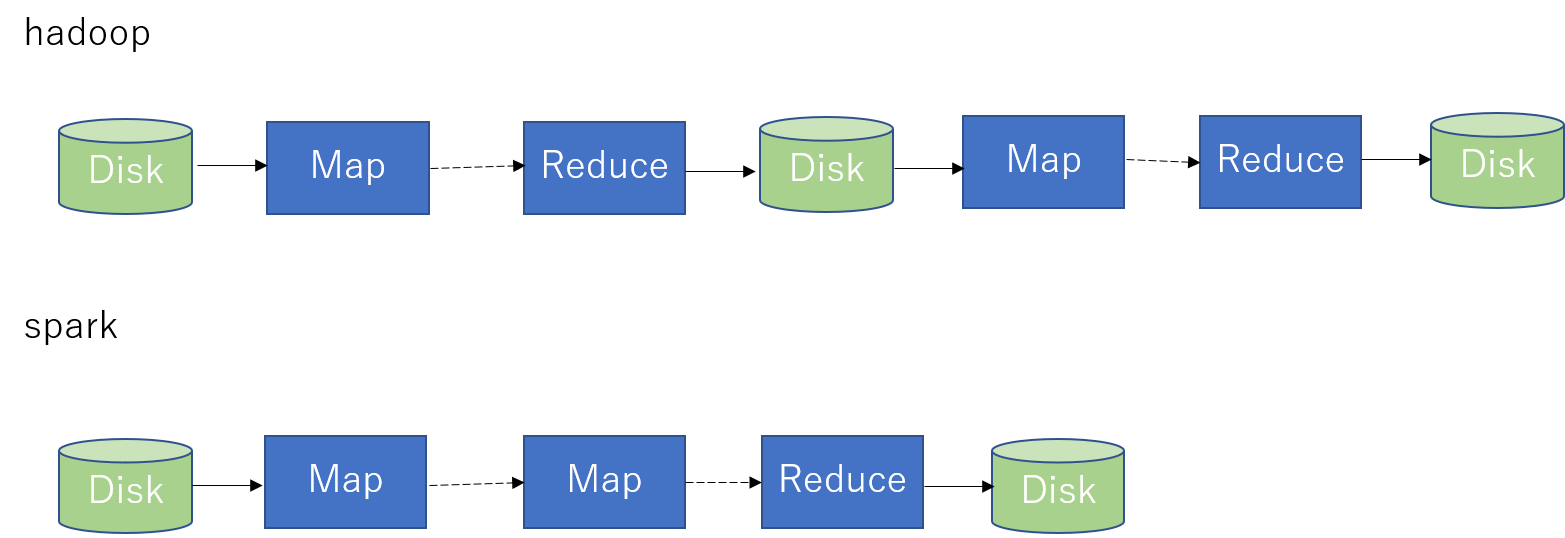
\includegraphics[scale=0.3]{figure/compare-hadoop-spark.png}}
  \caption{comparison of Hadoop and Spark processing methods}
  \label{fig:compare-hadoop-spark}
\end{figure}

\subsubsection{RDD}
RDD(Resident Distributed Data)\cite{zaharia2012resilient} is data structures that can be processed in parallel in Spark, and Spark performs distributed processing by processing against RDD.
There are two types of processing that can be performed on RDDs: Transformation, which transforms the RDD, and Action, which computes the result from the RDD.
Processes such as Map and Filter are Transformation, while Collect and Count are Action.
Transfromation processing for RDDs is not performed immediately, but rather in the form of a delayed evaluation that is processed all at once when the Action is called.

Taking WordCount in Fig.\ref{fig:dag} as an example, the map, flatmap and groupbykey correspond to TransFormation, and the collect corresponds to Action.
map is not actually processed at the stage when this is called, but when collect is called, all the processes are executed at once. 
To achieve this latency evaluation, Spark generates a graph called DAG (Directed acyclic graph) to achieve this delay evaluation.

\begin{figure}[htbp]
  \centerline{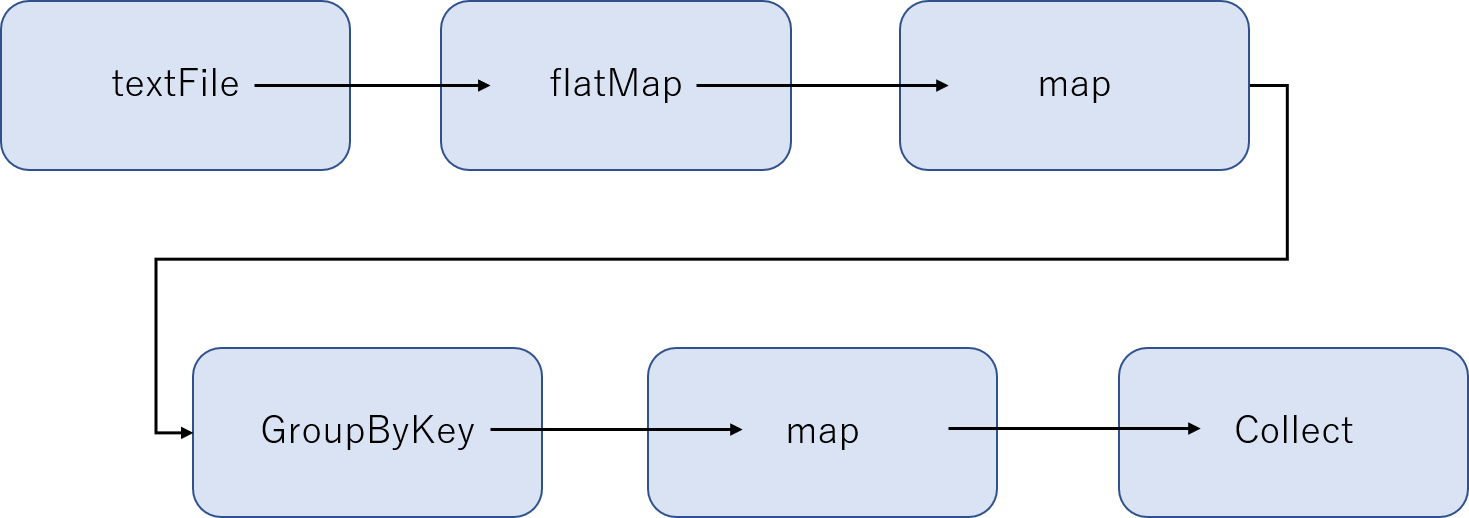
\includegraphics[scale=0.3]{figure/dag.png}}
  \caption{DAG in WordCount}
  \label{fig:dag}
\end{figure}

\subsubsection{DAG}
A DAG is a lineage diagram of an RDD that is generated when an Action is invoked.
RDDs maintain information about their parent RDDs. When an Action is called, the flow of processing can be obtained by tracing backward through the RDD.
This DAG is treated as one job, and each spark executor executes the job.
This allows MapReduce processing to be done all at once in memory.
In addition, by storing only this In addition, by storing only this DAG on the disk, the same data can be generated again in the event of a failure, thereby increasing This enhances fault-tolerance.

Fig.\ref{fig:dag} shows an example of a DAG generated by WordCount.
First, textFile reads data as RDDs from a file on disk in which words are recorded.Second, the combination of the word and the list of occurrences is created by map, flatmap, and groupbykey.Finally, the lists created by map are summed and the result is output by collect.
Each executor collectively executes a series of flows based on this DAG.
Spark is often used for machine learning and graph processing. These applications often have a loop structure that repeats the same process, and the same data may be used in each loop.
Spark caches such repeatedly used data to reduce disk access and computation time.
Fig.\ref{fig:dag_pr} shows PageRank's DAG as an example of a loop-structured application.

\begin{figure}[htbp]
  \centerline{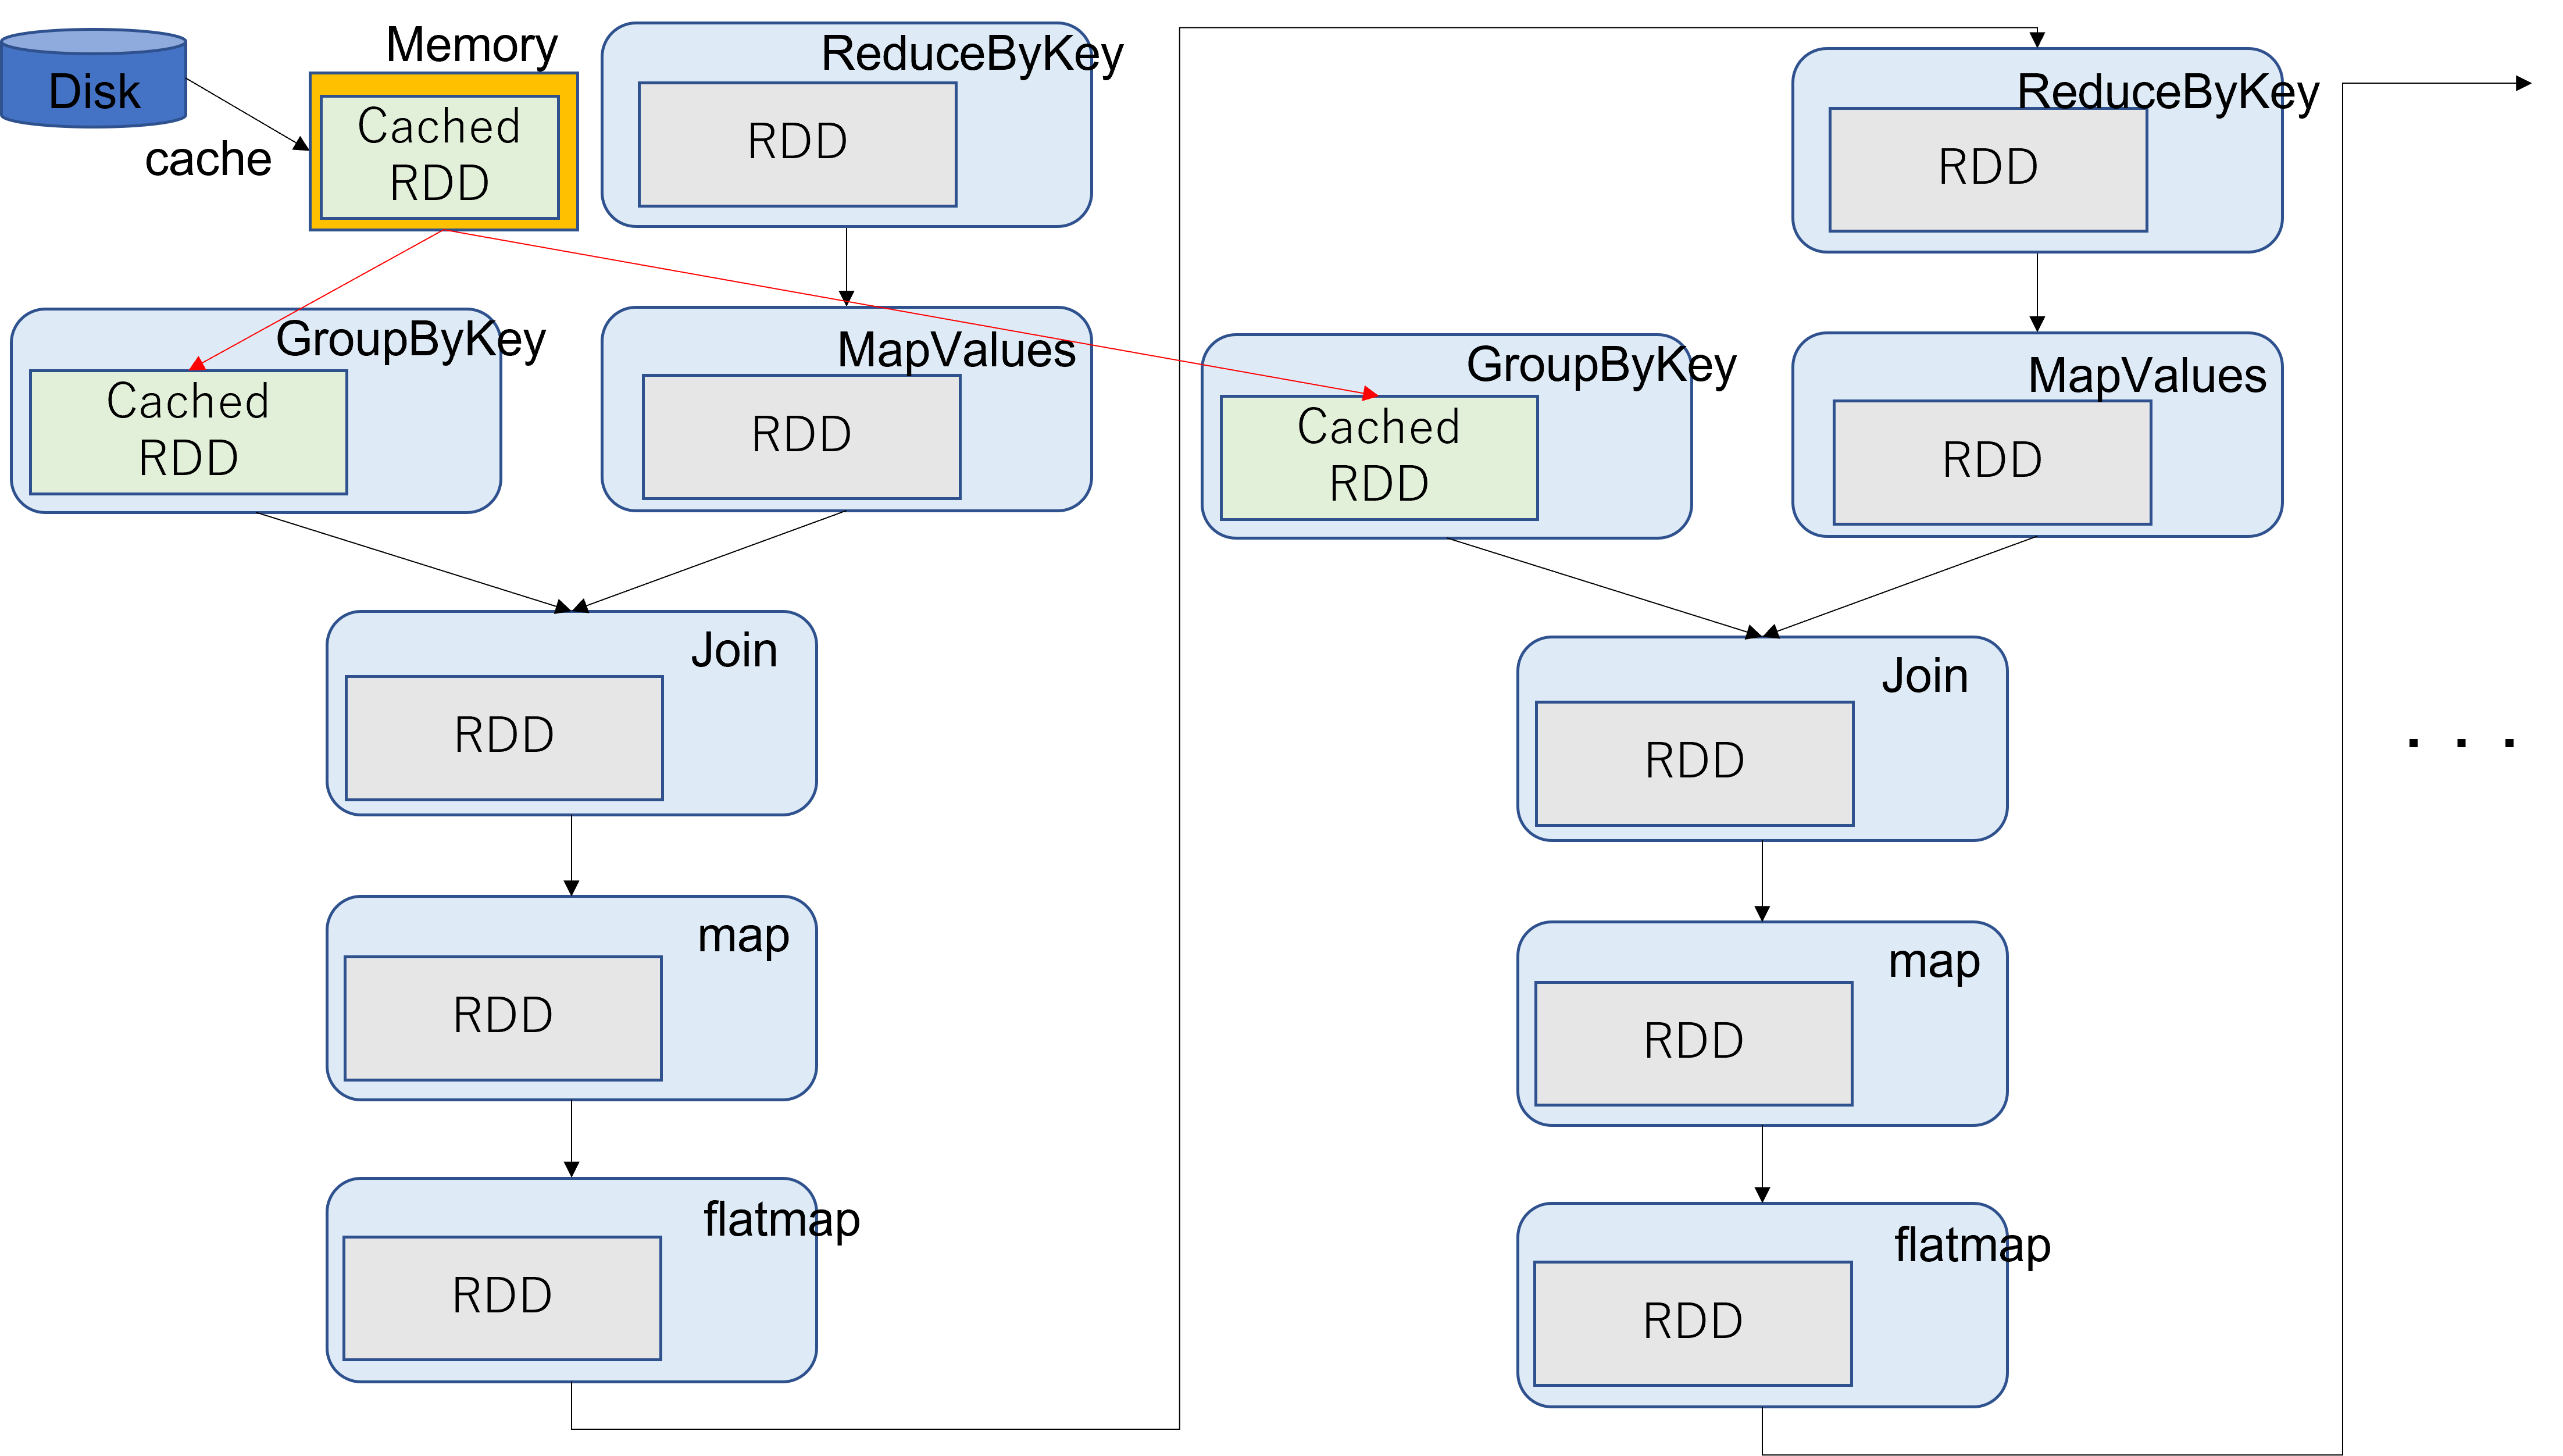
\includegraphics[scale=0.25]{figure/dag_pr.png}}
  \caption{DAG in PageRank}
  \label{fig:dag_pr}
\end{figure}

\subsubsection{spark memory management}
The memory structure of Spark is shown in Fig. StorageMemory and ExecutonMemory are the main processing areas of Spark.
StorageMemory is an area where cached RDDs and other long-lived objects are stored, while ExecutionMemory is an area for executing Spark tasks and is used for short-lived objects such as intermediate data. 
The sizes of StorageMemory and ExecutionMemory are not clearly defined, and the boundaries of the areas shift depending on the situation.
UserMemory and ReservedMemory is an area reserved for user data and internal metadata other than Spark processing.

\begin{figure}[htbp]
  \centerline{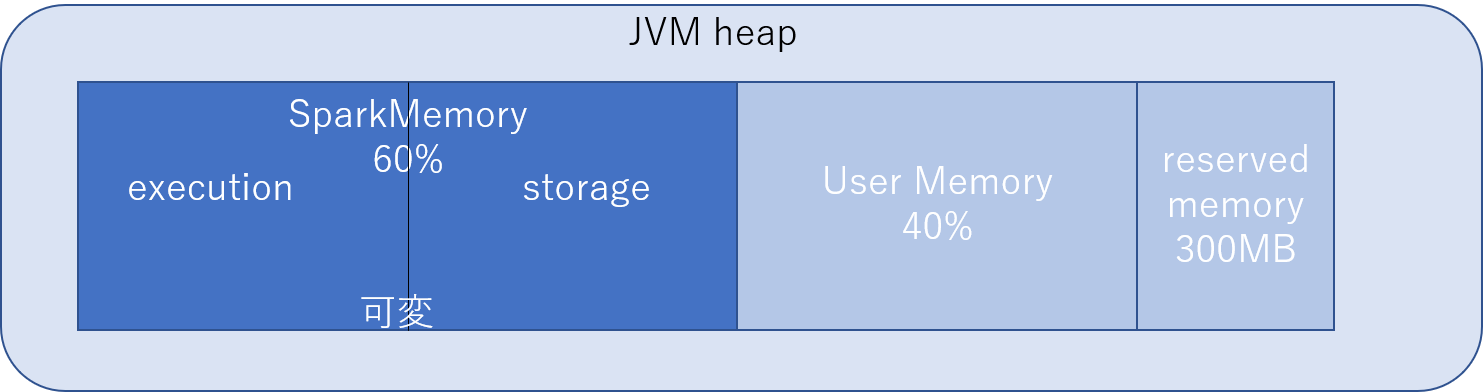
\includegraphics[scale=0.25]{figure/spark-memory-management.png}}
  \caption{spark memory management}
  \label{fig:spark-memory-management}
\end{figure}

\subsection{Hugepages} 
In this paper, we try to answer the following question: \emph{How
effective is the hugepage feature to Apache Spark applications?}

In-memory distributed processing frameworks such as 
Apach Spark use huge amounts of memory, so address translation is expected to take time.
In addition, applications running on Apache Spark are often structured to cache large amounts of data and access it repeatedly, so the benefits of hugepage are expected to be significant.
However, the effect of hugepages in an in-memory distributed processing framework is not clear, and it is not known how Spark memory structure affects hugepages.

There are two types of hugepage allocation in the current Spark standard: allocation entire and no hugepage.
This can be selected as an option when starting the JVM.
If there are no hugepage, the application will run on normal pages without using hugepage. In the case of allocation entire, when allocating memory on the JVM, a hugepage usage flag is given to all pages, and THP, Linux's hugepage allocation mechanism, allocates hugepage. Thus, the entire memory of the application running on the JVM becomes a hugepage.
Thus, Apache Spark allows only oll or nothing selection for hugepage allocation, and does not take into account Spark memory layout. In addition, THP has problems such as memory bloat and CPU occupancy for compaction, and if all memory is used for hugepage, a large memory bloat will occur.

\subsection{Previous Approaches}
Ingens\cite{kwon2016coordinated} is a mechanism for efficient hugepage management that solves the problems of increased latency and memory bloat that exist in hugepage.
Ingens improves performance by monitoring hugepage utilization and access frequency and allocating them at appropriate times.
Also, The illuminator is a hugepage management mechanism to solve fragmentation problems due to memory pollution.
Illuminator\cite{panwar2018making} explicitly manages hybrid regions with a mix of movable and unmovable pages to reduce memory movement overhead and improve performance.
These mechanisms target the management of hugepage in the OS as a whole, and hugepage management tailored to the characteristics of distributed processing frameworks has not been studied.
In addition, Ingens uses Spark as one of the workloads in the experiment, but only compares execution times and memory usage in THP and Ingens, and does not provide sufficient comparison with the case without hugepage or a detailed discussion of the effect hugepage had on Spark.

HotTub\cite{lion2016don} has focused on the JVM warm-up time as a bottleneck in distributed processing frameworks, and has improved performance by reducing warm-up time by using the JVM in different ways.
There has been much research on GC suitable for distributed processing systems\cite{nguyen2016yak, lu2016lifetime, gog2015broom, nguyen2015facade}, and Yak\cite{nguyen2016yak} has improved performance by combining generational GC and region-based GC, focusing on object characteristics with different lifetime in distributed processing systems.
Yak has significantly reduced GC time with Hadoop, GraphChi\cite{kyrola2012graphchi}, and Hyracks\cite{borkar2011hyracks}.
Since Spark uses a lot of memory, the cache hit ratio has a significant impact on performance, and research has been conducted to optimize the memory cache \cite{yu2017lrc, xu2016memtune, li2022intermediate, yu2017lrc, xu2020dag}.
In these studies, cache hit ratio was improved by cache management that takes advantage of Spark's object characteristics.
Various other studies on distributed processing systems have been conducted to improve Disk I/O\cite{zhang2018riffle}, reduce object serialization time\cite{nguyen2018skyway}, and reduce GC overhead\cite{ieee2015Xu, maas2016taurus}. However, these studies do not assume the use of hugepage, and the relationship between hugepage and distributed processing frameworks is still unclear.

\section{Methodology}
\subsection{Hugepage Allocation}
To investigate the effect of hugepages on Spark, we experiment with three hugepage allocation 
policies: 1. no hugepage, 2. allocation entire, and 
3. partial allocation(only the StorageMemory to Spark), and measure and compare the execution times.
With no hugepage, no hugepage related options are specified in the JVM options, 
and the base page is used by the JVM as a whole. With allocation entire, 
the JVM options specify the use of hugepages and the JVM as a whole uses hugepages. 
In partial allocation, By specifying the use of hugepages in the improved JVM, only 
StorageMemory objects are allocated as hugepages, and the rest are allocated as base pages. 
StorageMemory is an area such as a cache that is accessed repeatedly over a long period of time and where a large number of huge objects are stored. Therefore, StorageMemory is considered to be an area that benefits greatly from the speedup in address translation, which is one of the advantages of hugepages.
In this experiment, hugepage is allocated only to StorageMemory, and the effect of hugepages due to differences in object characteristics inside Spark's memory is verified. 

\subsection{Target Application}
To make it easier to understand the effect of allocating a hugepage to StorageMemory only, we prepared a microbenchmark with many accesses to StorageMemory. And 10 benchmarks used in the real world. benchmarks that are used in the real world. We run these benchmarks to investigate the effect of fusee pages in Spark.
\subsubsection{Micro Benchmark}
In this paper, the hugepage allocation to StorageMemory only is performed and compared with the allocation to no allocation or to the entire SparkMemory.
Page allocation to StorageMemory only, and compare it with the case of no allocation or allocation to the entire SparkMemory. 
We created a microbenchmark with frequent accesses to StorageMemory in order to easily understand the behavior and effects of the allocation. The behavior of the microbenchmark is shown below.
\begin{enumerate}
	\item Prepare a 4KB dummy object
	\item An array of dummy objects is created and cached. This will be stored in StorageMemory.
	\item Access to all objects in the array
	\item 3 repeated a certain number of times
\end{enumerate}
By accessing 4KB at a time, TLB misses are increased, making it easier to understand the effect of the hugepage allocation. 
\subsubsection{Real World Benchmark}
In the experiment, we ran the 10 real-world benchmarks shown in Table 4.1. The benchmarks are workloads that are actually used on Spark, such as machine learning and graph processing.
Kmeans, LogisticRegression, SVD++, LineareRegression, and GMM are benchmarks with little shuffling, large cached data, and high load on StorageMemory.
Conversely, PageRank and GBT are benchmarks with a high amount and number of shuffles and a high load on ExecutionMemory.
For the remaining ALS, SVM, and TC, both cache data and shuffle volume are reasonably large,
Both StorageMemory and xecutionMemory are used in this benchmark.
\subsection{Allocation Hugepages to Storage Memory}
Figure 4.2 is a schematic diagram of the mechanism for allocating hugepages on an object-by-object basis. For implementation, Apache Spark 3.2.0 and OpenJDK 11 modifications.
In Java, objects are created the new instruction.
In addition to the new instruction, this study implements the hp\_new instruction in the JVM to generate objects in a hugepage.
It also implements instructions that generate objects with the corresponding hugepage, such as the hp\_newarray instruction that generates arrays.
First, HugepageRegion was added to the JVM for implementation.
G1GC, the standard GC of OpenJDK11, divides and manages memory in units called regions. Under normal circumstances, all regions are either all hugepages or all base pages, since hugepages may or may not be used by each JVM.
This time, in order to select the use of the hugepage for each object, the hugepage Region and the base page Region are divided and managed separately. 
The first time the hp\_new instruction is called, it selects a region that has never been used from the free list that stores normal regions, moves it to the free list dedicated to the HugepageRegion, and adds the MADV\_HUGEPAGE advice via the madvise system call [43]. 
This allows memory to be allocated as a hugepage when Region is used.
At this time, if it is a used Region that has been used for other purposes and then returned to the free list, it cannot be allocated directly as a hugepage because the memory has already been allocated as a base page.
Therefore, regions that have never been used is selected first.
When the hp\_new instruction is called, allocation is performed from HugepageRegion, otherwise from the normal Region, and when the Region is full, the free list of the normal Region is moved to free list of the HugepageRegion in the same manner. 
In addition, When returning a used HugepageRegion, reuse the HugepageRegion by returning it to the free list dedicated to HugepageRegion.
This allocates the new instruction to the base page and the hp\_new instruction to the giant page. This allows selection on an object-by-object basis of whether to use the hugepage or not.

As an additional twist, HugepageRegion is set to the Old generation from the beginning.
In the generation-specific GC of JVM, there are Young region where frequent GC is performed and Old region where few GC are performed. When a region is created, it is initially a Young region, and if it survives multiple GCs, it is changed to an Old region. 
In the case of the HugepageRegion, it is assumed that the stored objects will be used for a long period of time, like a cache. Therefore, by making it the Old region from the beginning, in the Young region GC can be avoided.

\begin{figure}
	\centering
	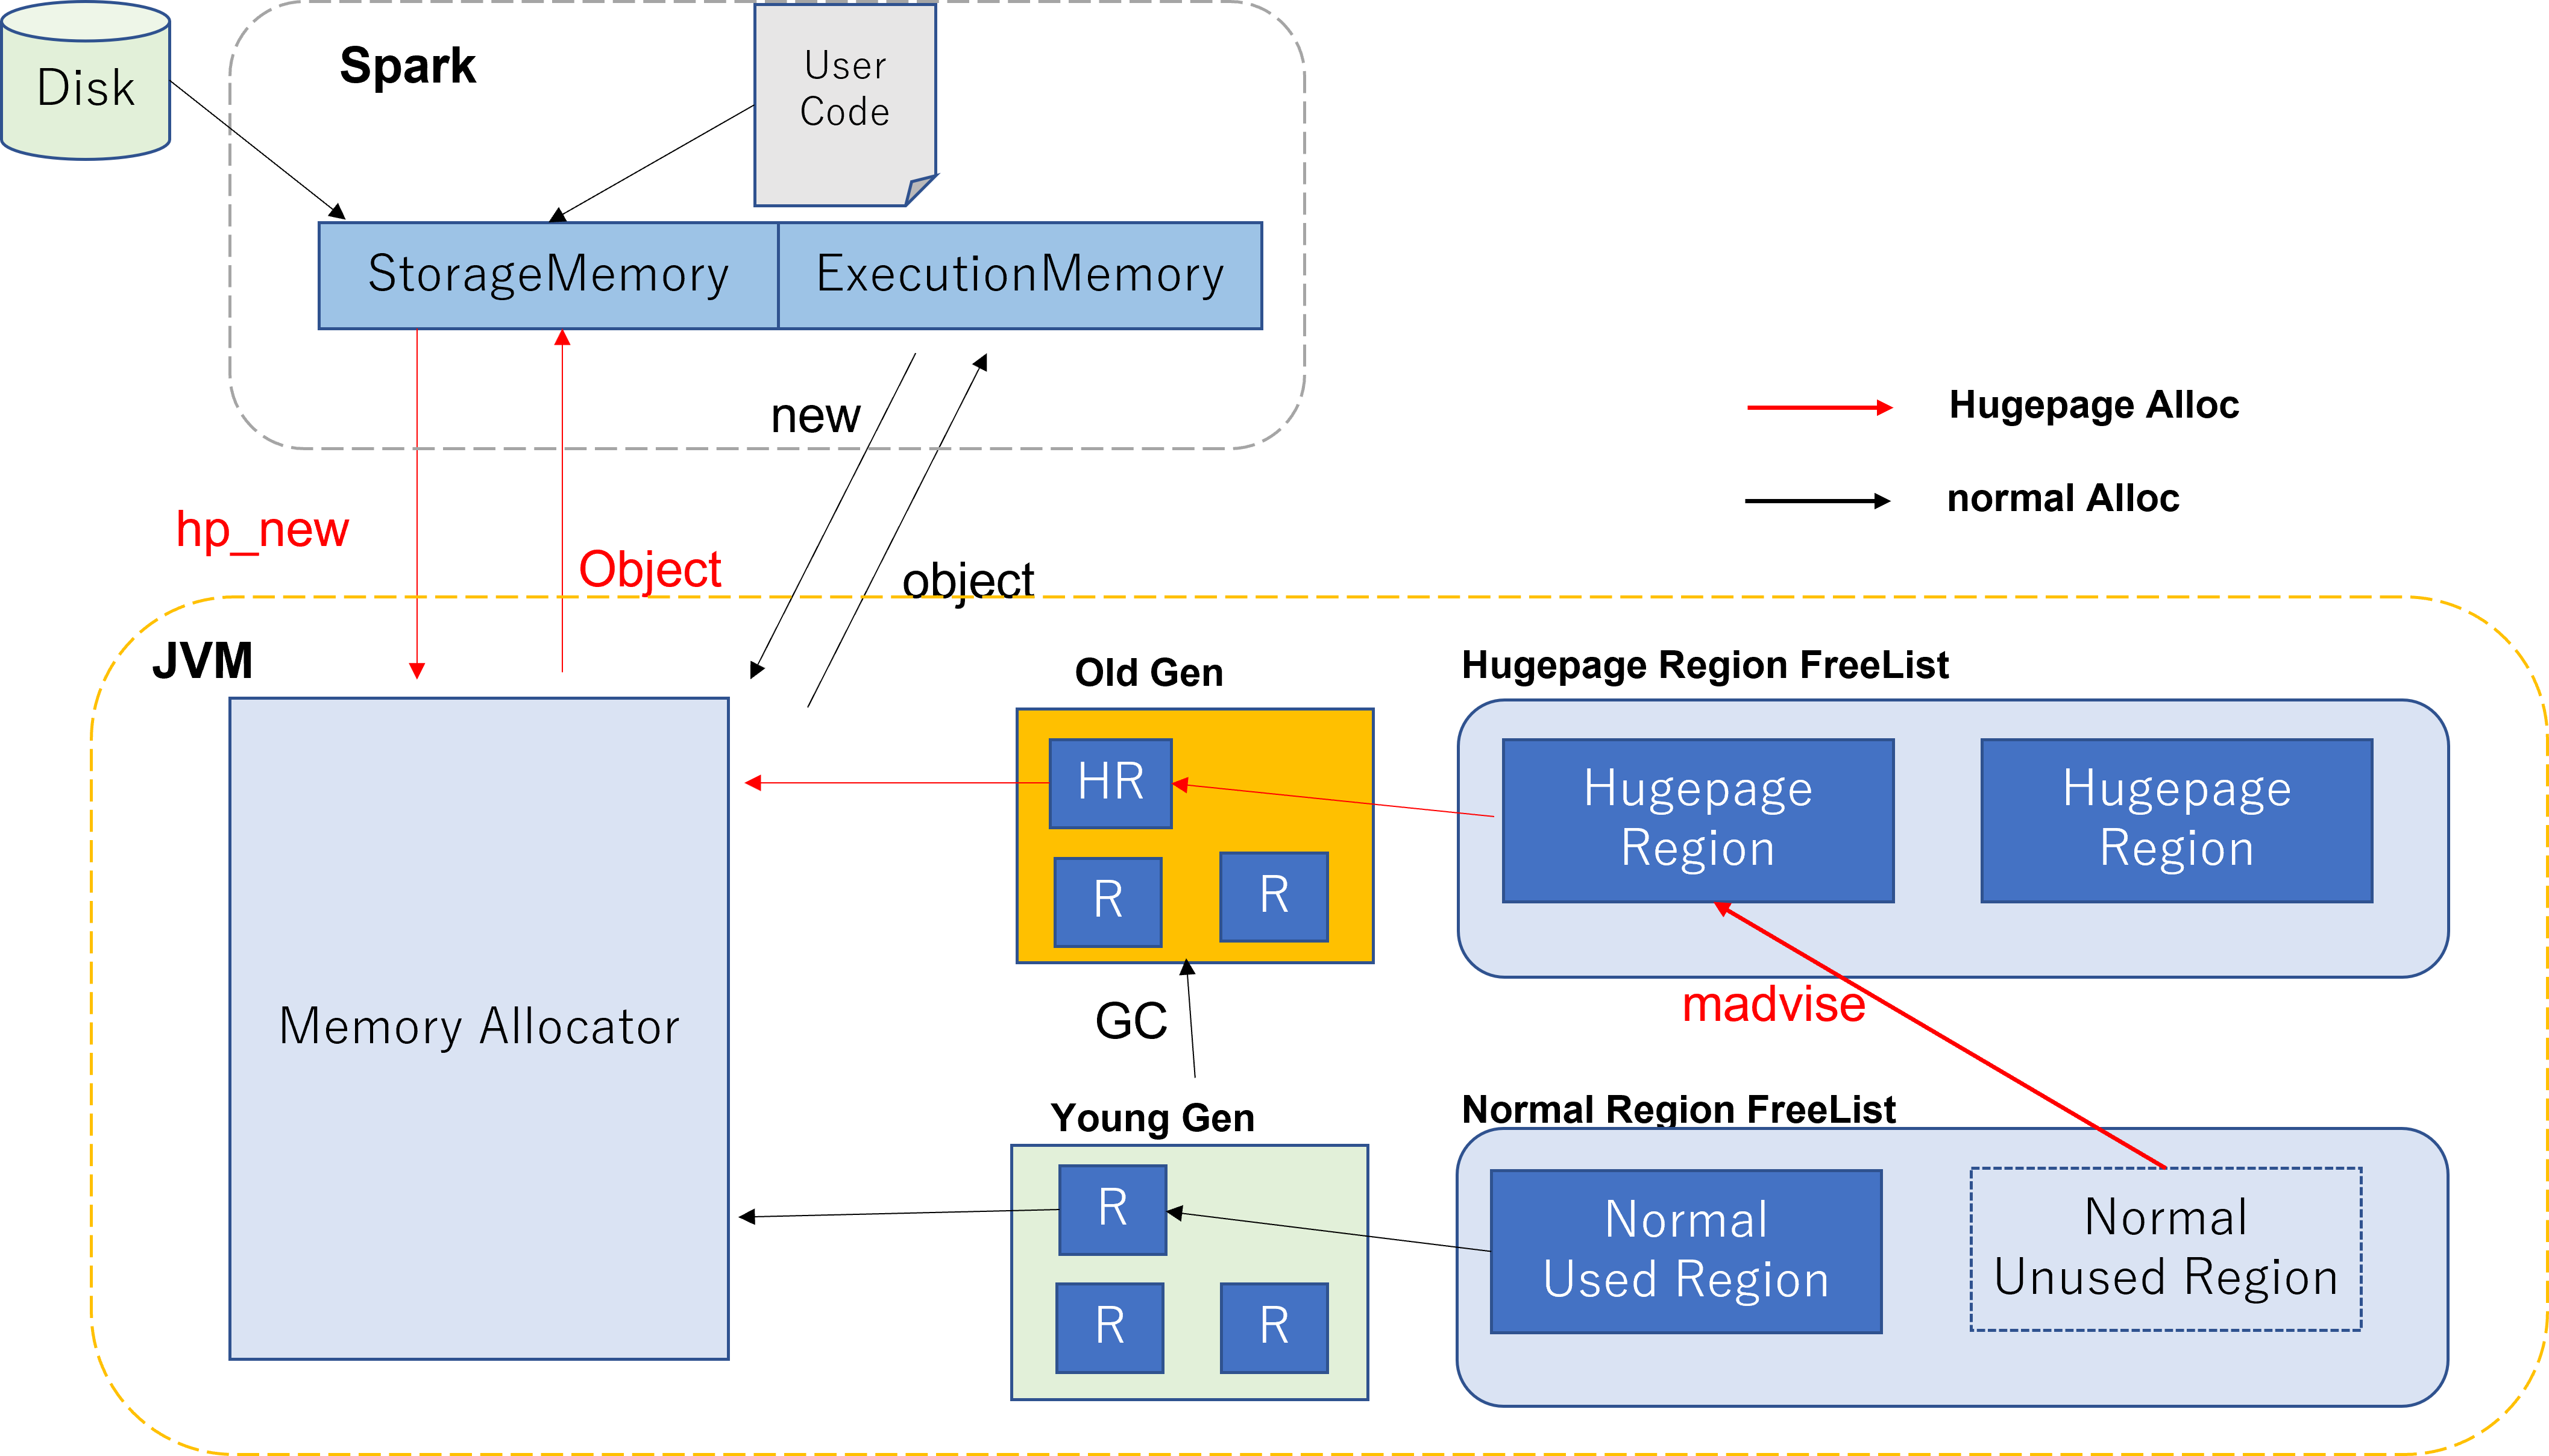
\includegraphics[scale=0.25]{figure/design.png}
	\caption{hugepage allocation per object}
	\label{fig:design}
\end{figure}

\section{Experiment}
\subsection{Experimental Environment}
Table \ref{tab:master-node} shows the performance of the machine used in the experiment and Table \ref{tab:spark-config} shows the Spark configuration.
In the experiment, two worker nodes were prepared and two executors were started in each worker node, making a total of four executors.
\begin{table}
	\caption{machine performance}
	\label{tab:master-node}
	\centering
	\begin{tabular}{ccc}
		\hline
		 & Master Node & Worker Node \\
		\hline
		CPU & Intel Xeon E5-2430 v2 & Intel Xeon E-2124 \\
		\hline
		Core & 4 & 4 \\
		\hline
		RAM & 32 & 64 \\
		\hline
		kernel & 5.4.0 & 5.4.0\\
		\hline
	\end{tabular}
\end{table}
\begin{table}
	\caption{Spark Configuration}
	\label{tab:spark-config}
	\centering
	\begin{tabular}{cc}
		\hline
		Executor & 4 \\
		\hline
		Core & 1 \\
		\hline
		Memory & 20GB \\
		\hline
	\end{tabular}
\end{table}
\subsection{Micro Benchmark}
The results of the microbenchmark runs are shown in Figure \ref{fig:mb}.
The execution time shows that partial allocation and entire allocation are reduced in execution time compared to those without allocation, indicating that the hue page is effective.
The overall allocation reduced execution time by about 5\%, while the partial allocation reduced execution time by about 12\%. It can be seen that partial allocation reduces execution time more.
Since the microbenchmark accesses StorageMemory frequently and ExecutionMemory is rarely used, so a partial allocation of hugepages to StorageMemory only is as effective as a entire allocation of husepages. 
In addition, It it thought that direct memory allocation to the Old region eliminates wasted GC in partial allocation, resulting in shorter execution time.
As for memory size, compared to no allocation, the maximum memory usage increased by about 1 GB for the overall allocation, indicating that memory bloat due to fragmentation, a disadvantage of HugePages, is occurring.
On the other hand, partial allocation, uses less memory than no allocation, resulting in a reduction in memory usage of approximately 4 GB. This may be due to the advantages of hugepages, such as page table compression, in addition to the fact that partial allocation uses fewer hugepages than total allocation, making fragmentation more difficult to occur.
\begin{figure}
	\begin{minipage}{0.5\hsize}
  		\centering
		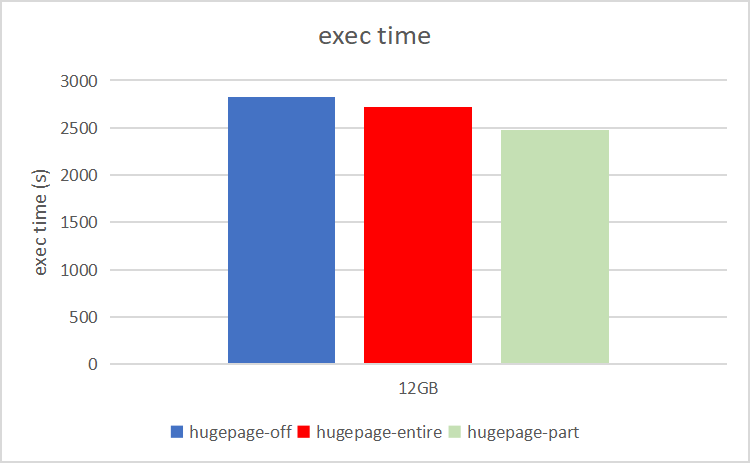
\includegraphics[scale=0.7]{figure/experiment_en/syuron/mb/exec_time.png}
	\end{minipage}
	\begin{minipage}{0.5\hsize}
  		\centering
		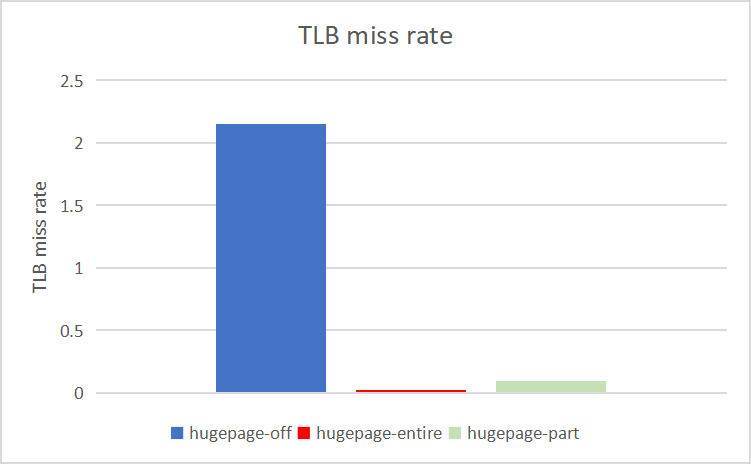
\includegraphics[scale=0.7]{figure/experiment_en/syuron/mb/tlb_miss.png}
	\end{minipage}
	\\
	\\
	\begin{minipage}{0.5\hsize}
		\centering
	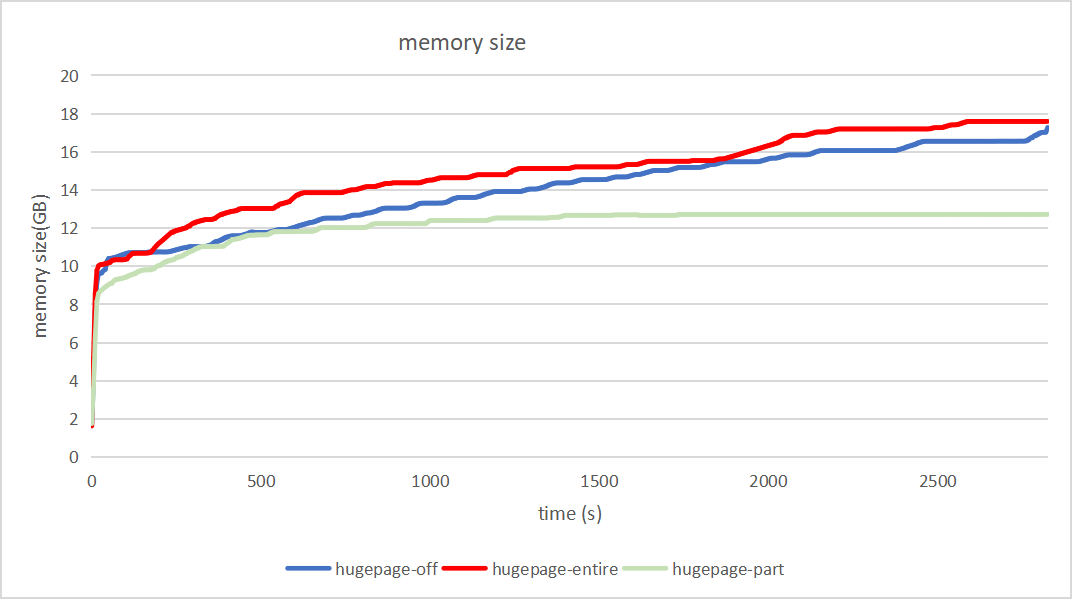
\includegraphics[scale=0.5]{figure/experiment_en/syuron/mb/memory_size.png}
	\end{minipage}
	\begin{minipage}{0.5\hsize}
		\centering
		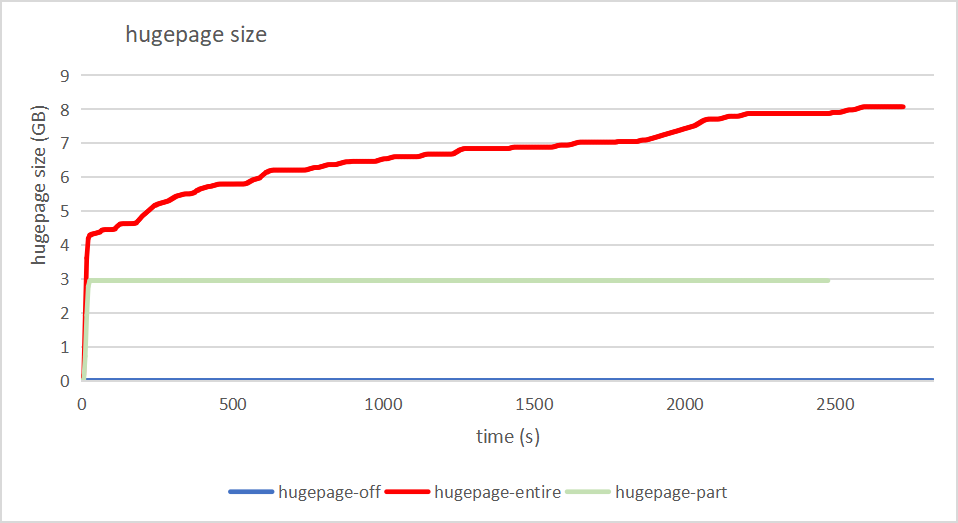
\includegraphics[scale=0.55]{figure/experiment_en/syuron/mb/hugepage_size.png}
	\end{minipage}
	\caption{experiment result of Micro Benchmark}
	\label{fig:mb}
\end{figure}
\subsection{PageRank}
The results of the PageRank runs are shown in Figure \ref{fig:pr}.
The execution time shows that the overall allocation greatly reduces the execution time by approximately 12\% compared to no allocation, while the partial allocation is equivalent to no allocation. This indicates that the effect  the hugepage on Execution Memory.
PageRank has a large read/write data size during shuffling, and the HashMap data prepared for shuffling generated in the Execution Meomory becomes large. It is thought that the increased access to this data has the effect of speeding up memory accesses, which is an effect of hugepage.
HashMap data is accessed randomly, unlike the sequential access of a byte array.
This causes many TLB miss, which are thought to be ameliorated by HugePages.
Unlike sequential accesses such as byte arrays, HashMap data is random access.
This causes many TLB errors, but it is thought that HugePages improving this situation.
partial allocation reduced execution time by only about 1\%.
This is due to the fact that in some allocations, hugepages are only allocated to StorageMemory,
It is believed that this is because the effect of Hugepages is relatively small in PageRank, where ExecutionMemory is more important.
The size of the hugepage in partial allocation is less than one-tenth of the entire allocation, which suggests that the hugepage is less effective.
Since memory is eventually used up to its maximum, the memory size is almost the same for all policies. However, up to about 1500 seconds, the memory size is smaller for partial allocation than for total allocation, thus reducing memory bloat. This indicates that the memory bloat becomes larger as more hugepages are allocated.

\begin{figure}
	\begin{minipage}{0.5\hsize}
  		\centering
		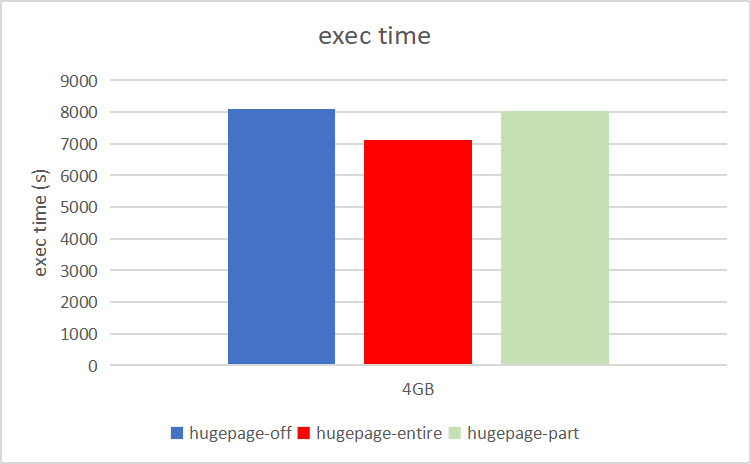
\includegraphics[scale=0.7]{figure/experiment_en/syuron/pr/exec_time.png}
	\end{minipage}
	\begin{minipage}{0.5\hsize}
  		\centering
		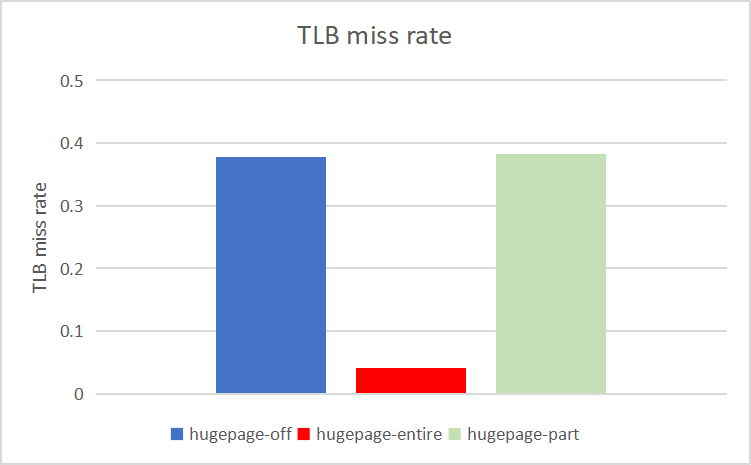
\includegraphics[scale=0.7]{figure/experiment_en/syuron/pr/tlb_miss.png}
	\end{minipage}
	\\
	\\
	\begin{minipage}{0.5\hsize}
		\centering
	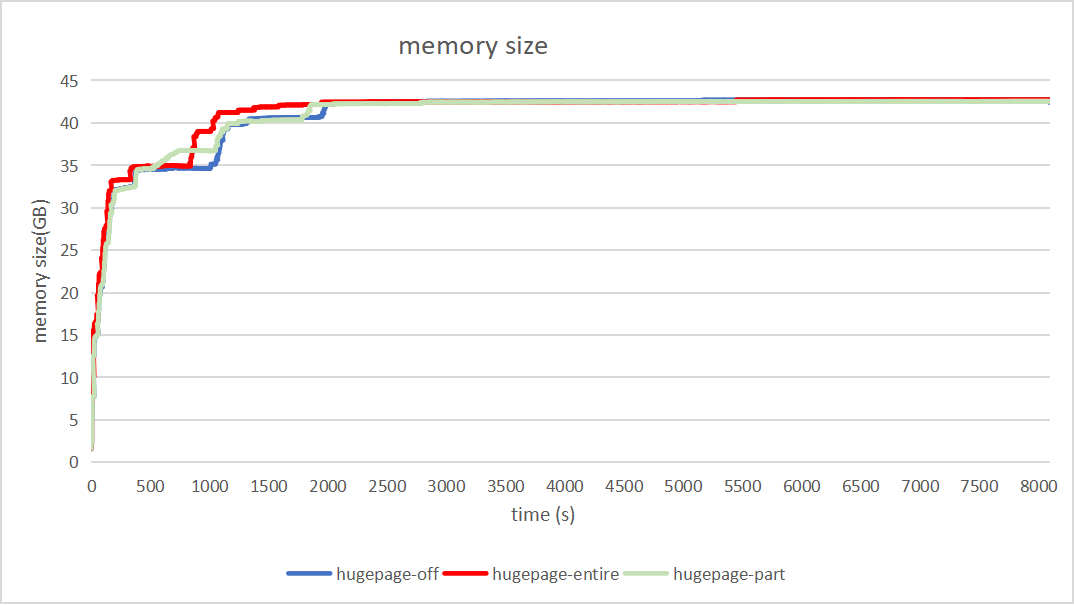
\includegraphics[scale=0.5]{figure/experiment_en/syuron/pr/memory_size.png}
	\end{minipage}mb
	\begin{minipage}{0.5\hsize}
		\centering
		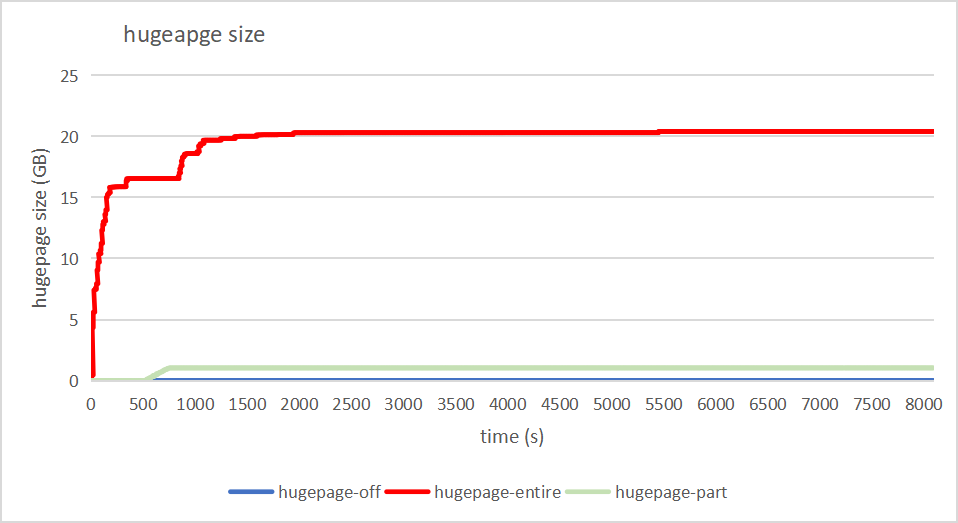
\includegraphics[scale=0.55]{figure/experiment_en/syuron/pr/hugepage_size.png}
	\end{minipage}
	\caption{experiment result of PageRank}
	\label{fig:pr}
\end{figure}
\subsection{Kmeans}
The results of the Kmeans runs are shown in Figure \ref{fig:kmeans}.
The execution time for the entire assignment was reduced by about 5\%, and that for partial assignment was reduced by about 3\%. 
This shows that the effect of hugepages reduces execution time, and that hugepages are effective even when allocated to only a part of the memory.
In kmeans, the effect is not as large as in the microbenchmark because the size to be cached is smaller than in the microbenchmark, but the amount of shuffling is small and the specific weight of StorageMemory is large, so it is clear that the fusee page is fully effective even with partial allocation.
The TLB miss rate shows that partial allocation does not reduce TLB misses as significantly as entire allocation.
This is thought to be due to speed improvements such as higher speed due to page table walk reduction other than TLB misses.
The same trend is observed in memory size as in the microbenchmarks.
While the overall allocation causes memory bloat, the partial allocation reduces memory usage more than the overall allocation.
\begin{figure}
	\begin{minipage}{0.5\hsize}
  		\centering
		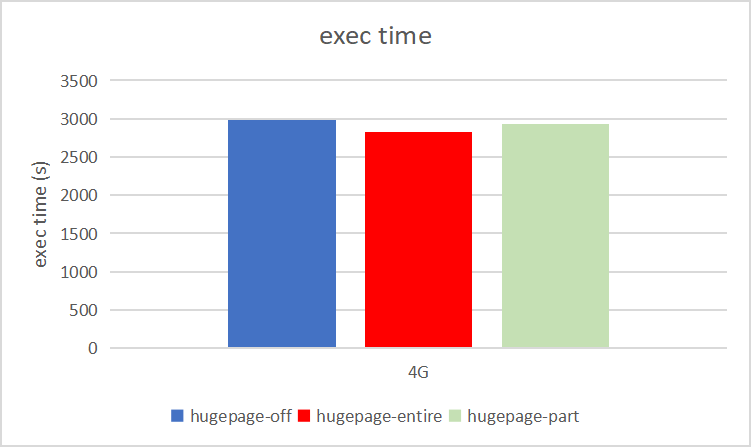
\includegraphics[scale=0.7]{figure/experiment_en/syuron/kmeans/exec_time.png}
	\end{minipage}
	\begin{minipage}{0.5\hsize}
  		\centering
		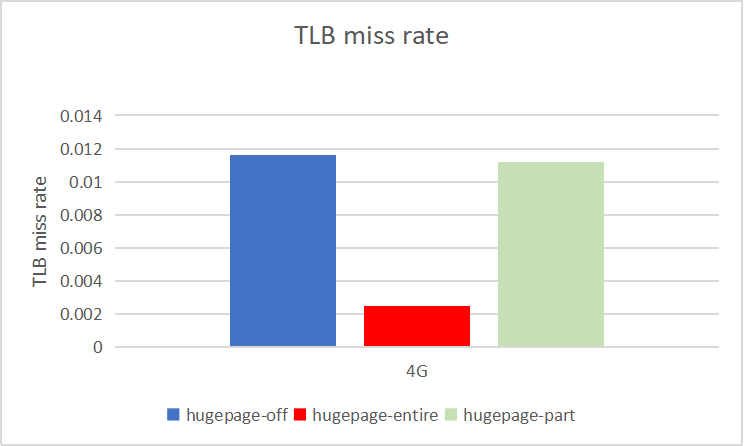
\includegraphics[scale=0.7]{figure/experiment_en/syuron/kmeans/tlb_miss.png}
	\end{minipage}
	\\
	\\
	\begin{minipage}{0.5\hsize}
		\centering
	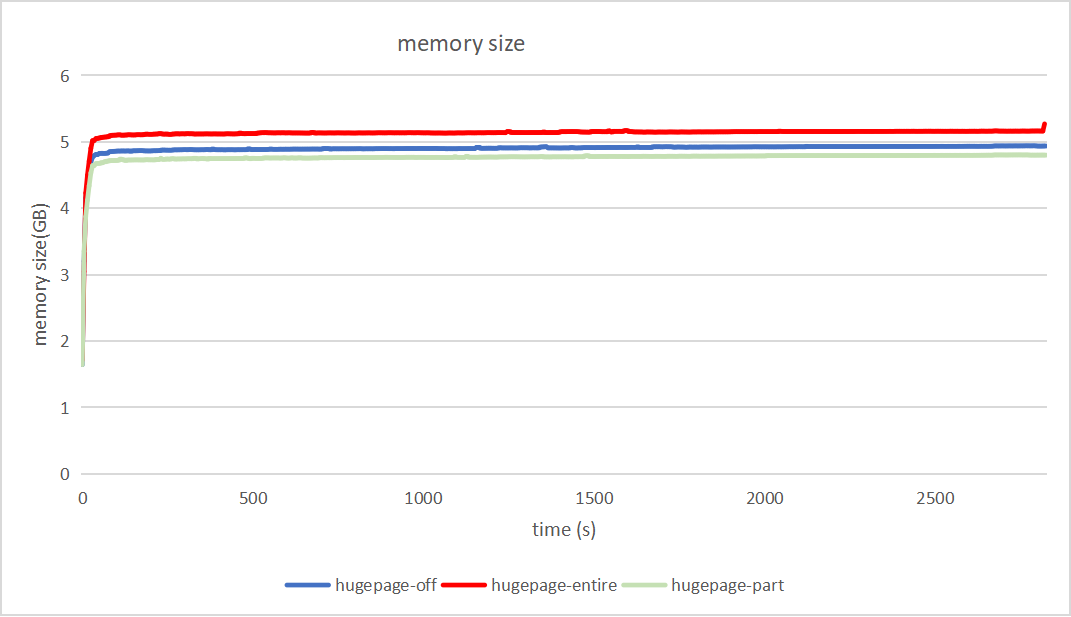
\includegraphics[scale=0.5]{figure/experiment_en/syuron/kmeans/memory_size.png}
	\end{minipage}
	\begin{minipage}{0.5\hsize}
		\centering
		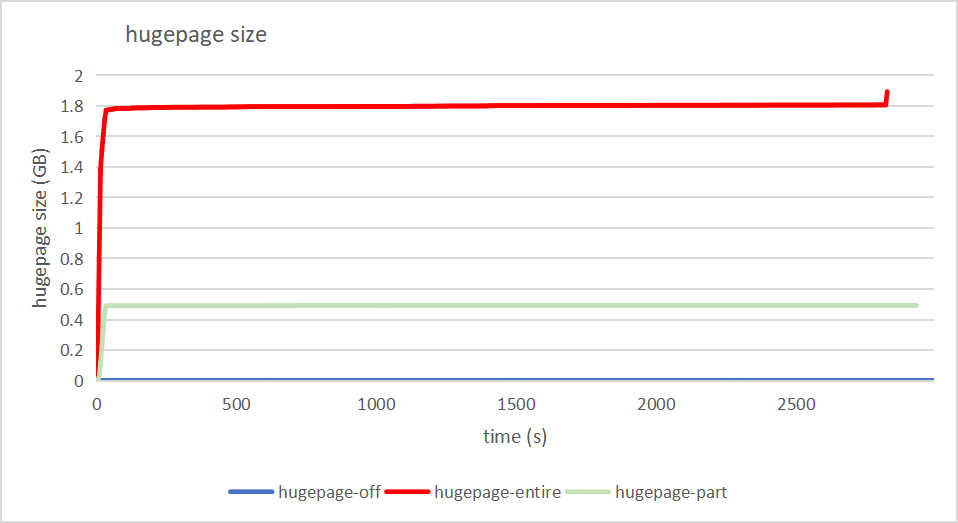
\includegraphics[scale=0.55]{figure/experiment_en/syuron/kmeans/hugepage_size.png}
	\end{minipage}
	\caption{experiment result of Kmeans}
	\label{fig:kmeans}
\end{figure}

\subsection{LogisticRegression}
The results of the LogisticRegression runs are shown in Figure \ref{fig:lr}.
The execution time is almost the same for entire allocation as for no allocation, and about 6\% shorter for partial allocation.
Since the cache size is large in LogisitcRegression and shuffling is not performed, the percentage of StorageMemory becomes high, and it is thought that the effect of the fuse page in StorageMemory is demonstrated, leading to speed improvement in partial allocation.
Another possible cause is the direct allocation of Old regions as described in the microbenchmark. 
The hugepage allocation size shows that the overall allocation allocates about five times as many fuse pages as the partial allocation.
However, the overhead of hugepage allocation outweighed the benefit due to the large number of accesses to the cache and the waste of hugepage allocation to the except of the StorageMemory, which may be the reason why the execution time could not be reduced.
The memory size is about 1.2GB for partial allocation compared to about 1.8GB for entire allocation, indicating that memory bloat is suppressed for partial allocation.

\begin{figure}
	\begin{minipage}{0.5\hsize}
  		\centering
		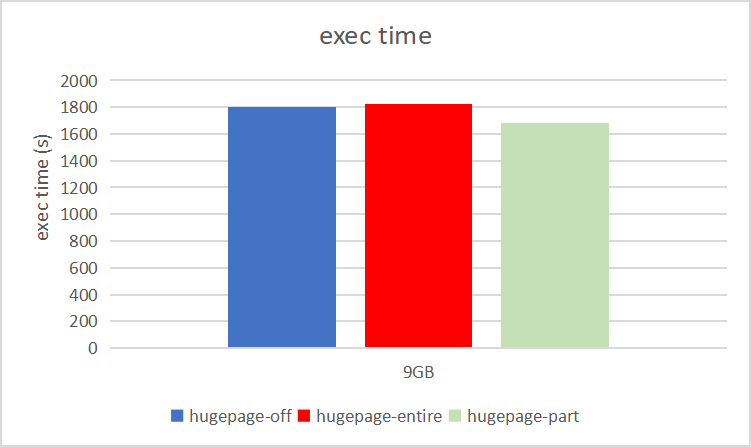
\includegraphics[scale=0.7]{figure/experiment_en/syuron/lr/exec_time.png}
	\end{minipage}
	\begin{minipage}{0.5\hsize}
  		\centering
		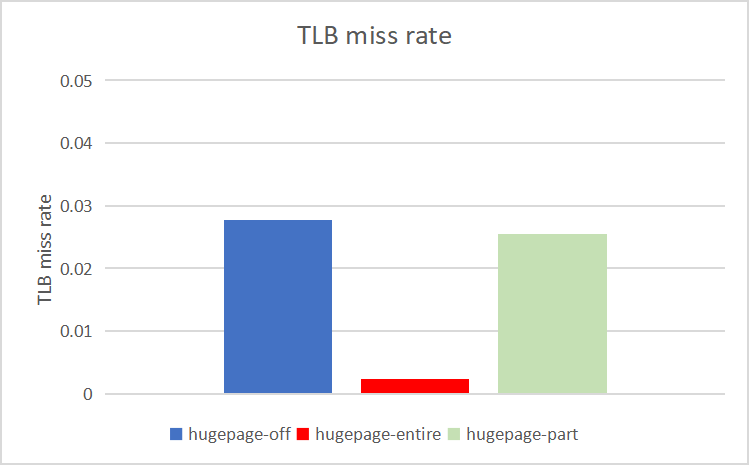
\includegraphics[scale=0.7]{figure/experiment_en/syuron/lr/tlb_miss.png}
	\end{minipage}
	\\
	\\
	\begin{minipage}{0.5\hsize}
		\centering
	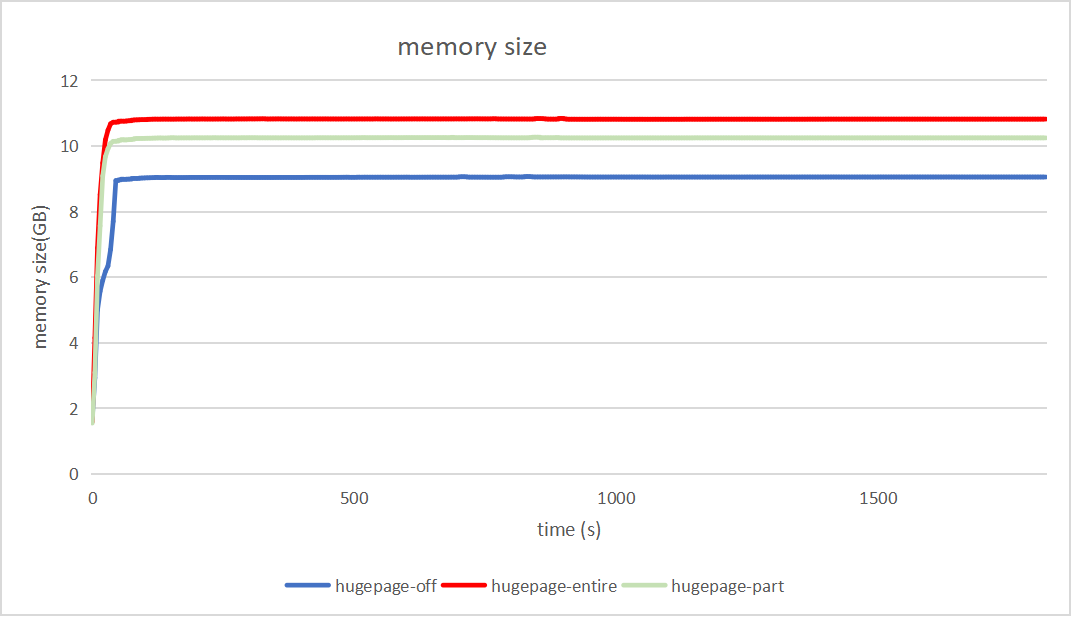
\includegraphics[scale=0.5]{figure/experiment_en/syuron/lr/memory_size.png}
	\end{minipage}
	\begin{minipage}{0.5\hsize}
		\centering
		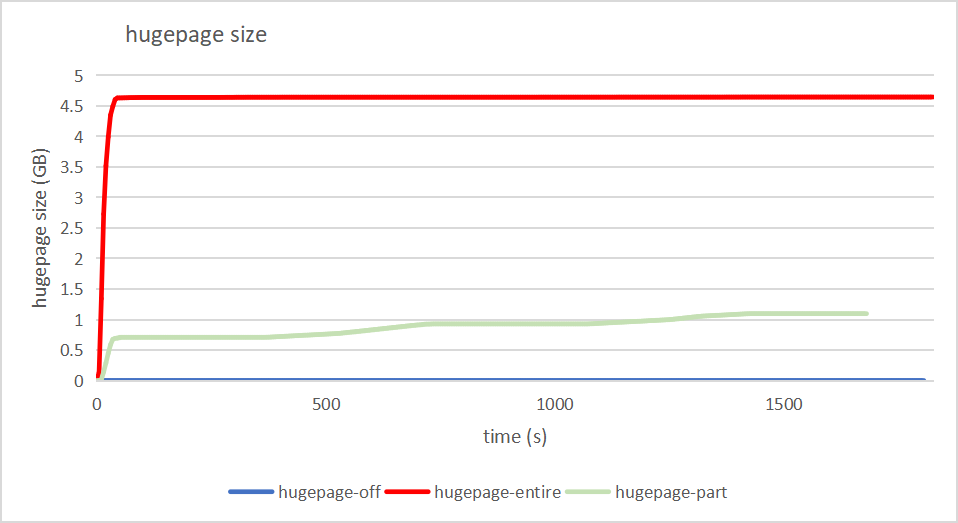
\includegraphics[scale=0.55]{figure/experiment_en/syuron/lr/hugepage_size.png}
	\end{minipage}
	\caption{experiment result of LogisticRegression}
	\label{fig:lr}
\end{figure}

\subsection{SVD++}
The results of the SVD++ runs are shown in Figure \ref{fig:svd}.
The execution time is reduced by approximately 6\% for entire allocation and approximately 5\% for partial allocation, indicating that the hue page effect reduces the execution time.
There was not much difference in execution time between partial and entire allocation, suggesting that the effect of the storage memory hugepage was effective.
Also, unlike the microbenchmark and LogisticRegression, the maximum memory is used, indicating that shuffling is done to a certain extent.
However, it is believed that access to data used in shuffling is low and access to cache data is concentrated, so that even partial allocation is sufficient.
memory size, with a maximum of 5.6GB for the entire allocation and 3.3GB for a partial allocation, and a large memory bloat is observed for the entire allocation with a large allocation of hugepages. 
\begin{figure}
	\begin{minipage}{0.5\hsize}
  		\centering
		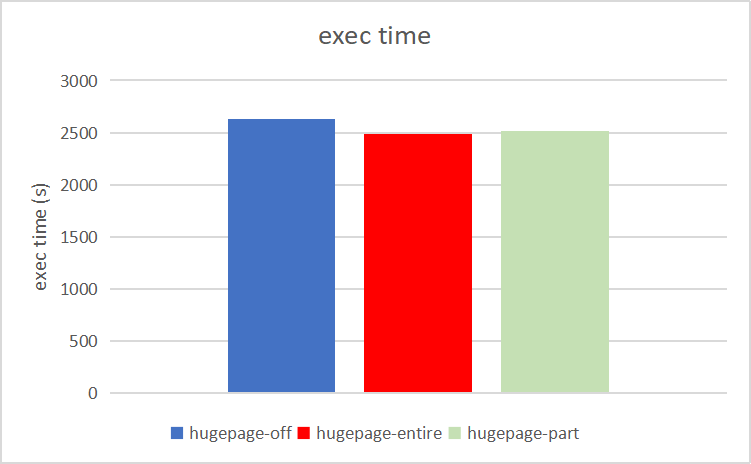
\includegraphics[scale=0.7]{figure/experiment_en/syuron/svd/exec_time.png}
	\end{minipage}
	\begin{minipage}{0.5\hsize}
  		\centering
		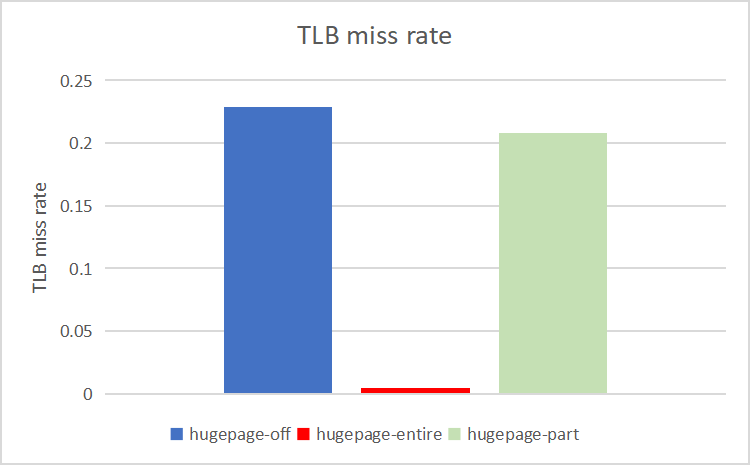
\includegraphics[scale=0.7]{figure/experiment_en/syuron/svd/tlb_miss.png}
	\end{minipage}
	\\
	\\
	\begin{minipage}{0.5\hsize}
		\centering
	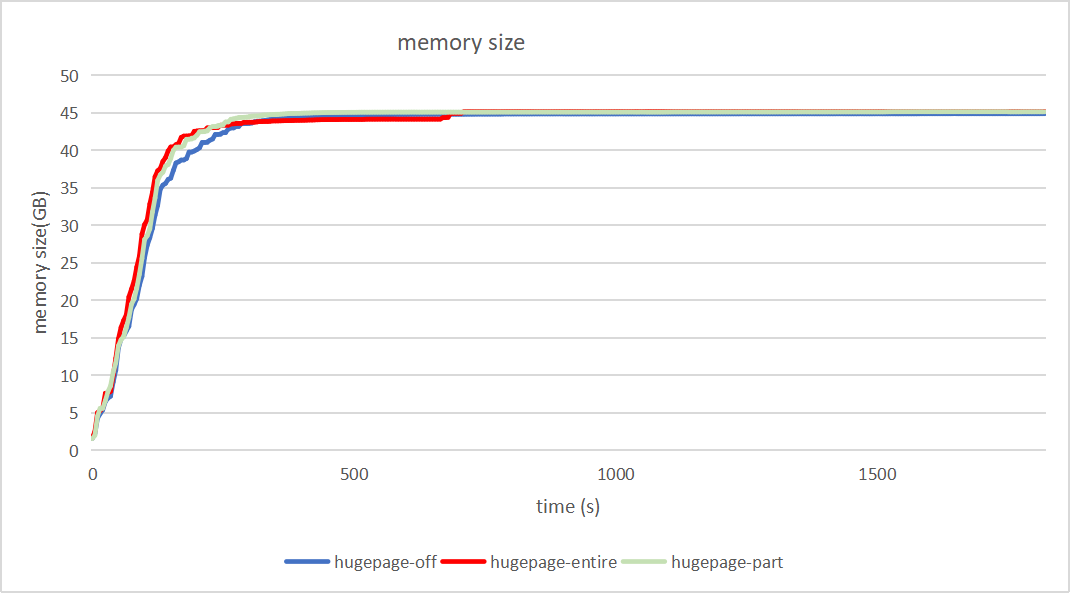
\includegraphics[scale=0.5]{figure/experiment_en/syuron/svd/memory_size.png}
	\end{minipage}
	\begin{minipage}{0.5\hsize}
		\centering
		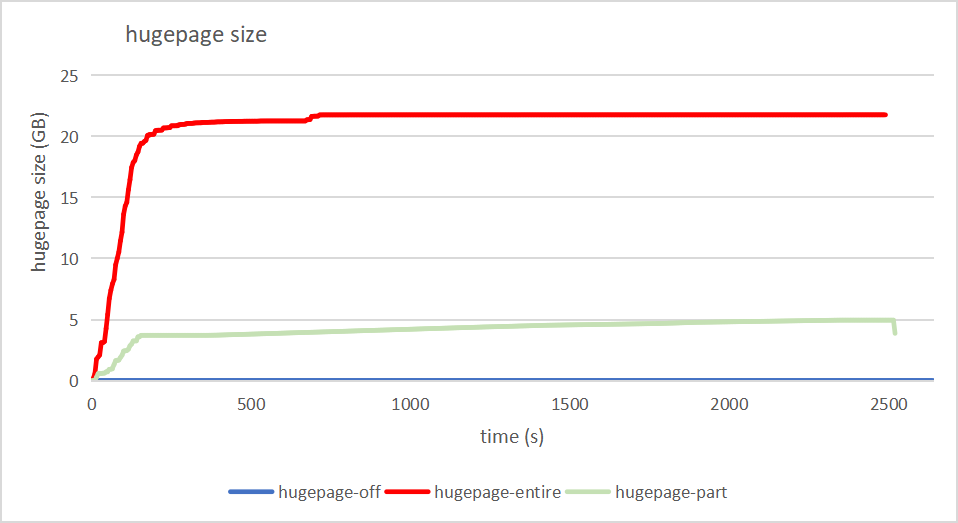
\includegraphics[scale=0.55]{figure/experiment_en/syuron/svd/hugepage_size.png}
	\end{minipage}
	\caption{experiment result of SVD++}
	\label{fig:svd}
\end{figure}
\subsection{LinearRegression}
The results of the LinearRegression runs are shown in Figure \ref{fig:lir}.
The execution time did not change for any of the policies, indicating that hugepage was not effect.
Looking at TLB misses, the entire allocation reduced the TLB miss rate by less than half, but the original TLB miss rate was as low as 0.07\%. Therefore, the actual reduction was as low as about 0.04\%, suggesting that the benefit of faster memory access due to TLB hits was small.
Another reason is that the execution time itself is shorter than in other benchmarks, which means that the time that can benefit from allocating hugepages is smaller relative to the overall execution time.
The memory size will eventually run out and there will be no difference between policies. However, during the execution, the memory is bloat to a maximum of 1.5 GB for the entire allocation and 2.5 GB for a partial allocation.
Even though the hugepage size is smaller for partial allocation than for entire allocation, the memory bloat is larger for partial allocation.
One possible reason for this could be the reduction of fragmentation due to memory compaction. The entire allocation has dozens of times more compact stalls than the partial allocation, and the execution time is about 1\% longer than the partial allocation in exchange for less bloat.
\begin{figure}
	\begin{minipage}{0.5\hsize}
  		\centering
		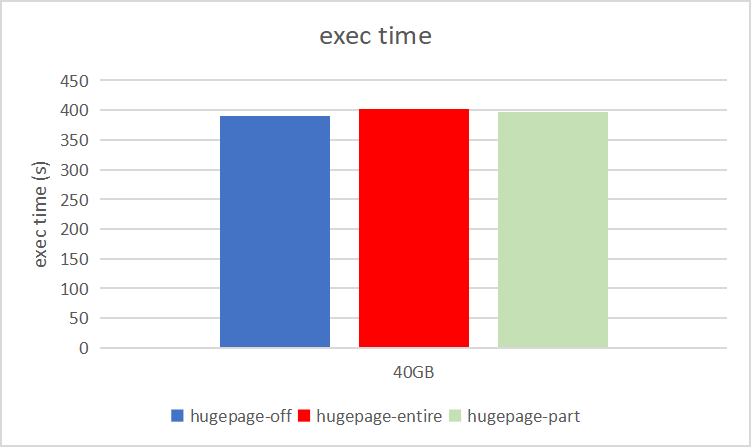
\includegraphics[scale=0.7]{figure/experiment_en/syuron/lir/exec_time.png}
	\end{minipage}
	\begin{minipage}{0.5\hsize}
  		\centering
		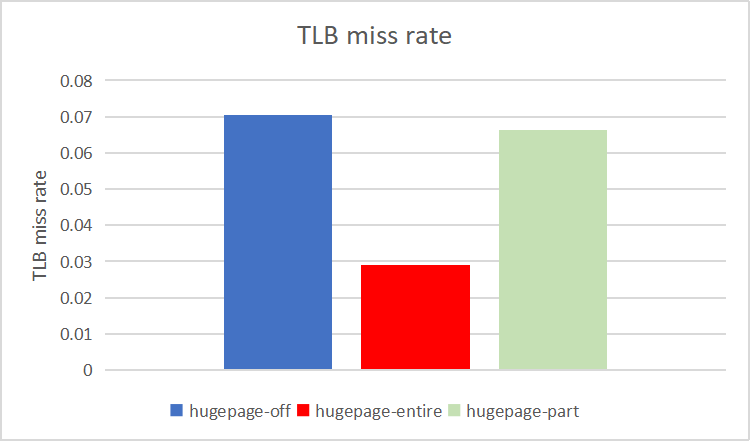
\includegraphics[scale=0.7]{figure/experiment_en/syuron/lir/tlb_miss.png}
	\end{minipage}
	\\
	\\
	\begin{minipage}{0.5\hsize}
		\centering
	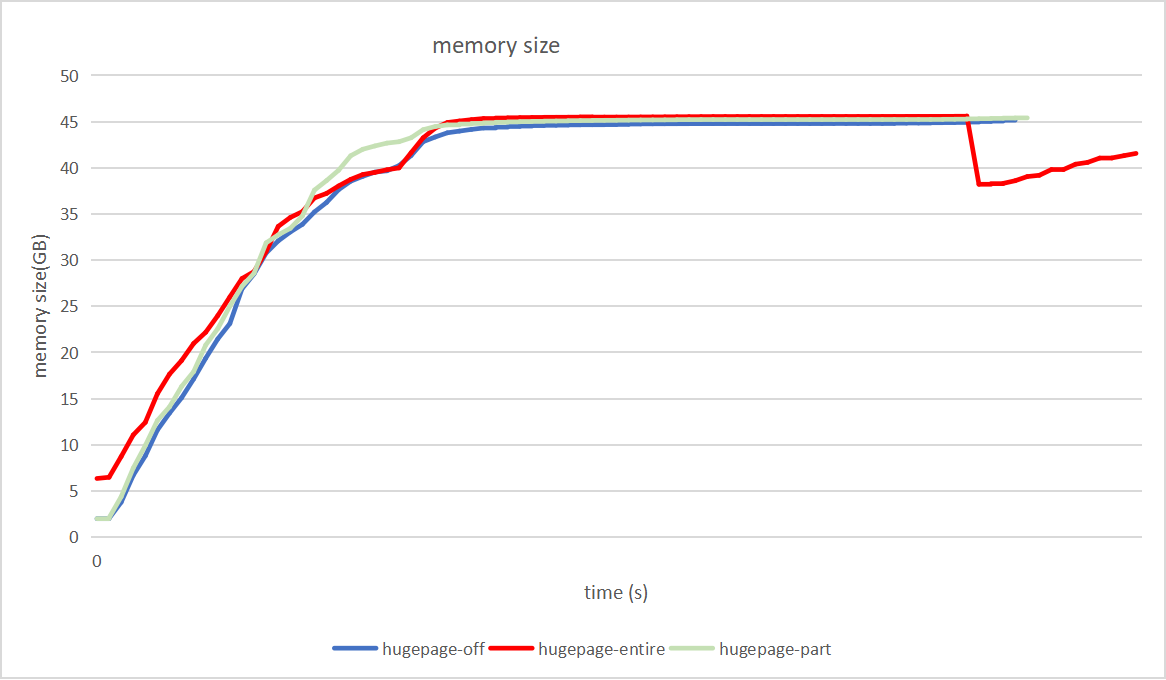
\includegraphics[scale=0.45]{figure/experiment_en/syuron/lir/memory_size.png}
	\end{minipage}
	\begin{minipage}{0.5\hsize}
		\centering
		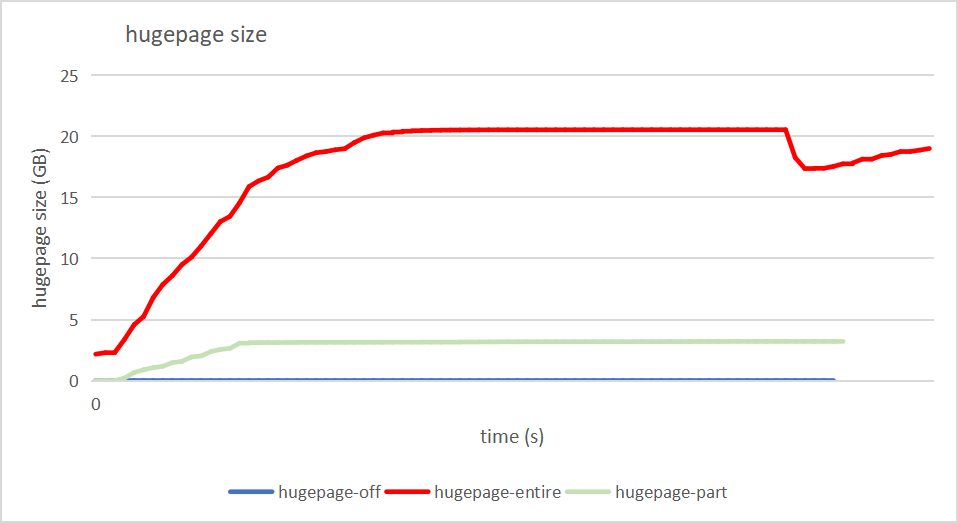
\includegraphics[scale=0.55]{figure/experiment_en/syuron/lir/hugepage_size.png}
	\end{minipage}
	\caption{experiment result of LinearRegression}
	\label{fig:lir}
\end{figure}
\subsection{GMM}
The results of the GMM runs are shown in Figure \ref{fig:gmm}.
Execution times are about the same for all policies, indicating that hue pages are less effective.
The reason may be that the original TLB miss rate is low (less than 0.01\%), so there is no speedup due to improved TLB hits, and the shuffle size is small, so the amount of access to ExecutionMemory is small.
In addition, the cache size is about 40 GB, which is very large, but the execution time is not reduced. From this is thought that the cache size is not always proportional to the benefit from the hugepage, and the number of cache accesses and the way they are done also play a role. 
The memory size is up to 8.8 GB for entire allocation and 4.5 GB for partial allocation, and memory bloat is suppressed by minimizing the allocation of hugepages in partial allocation.

\begin{figure}
	\begin{minipage}{0.5\hsize}
  		\centering
		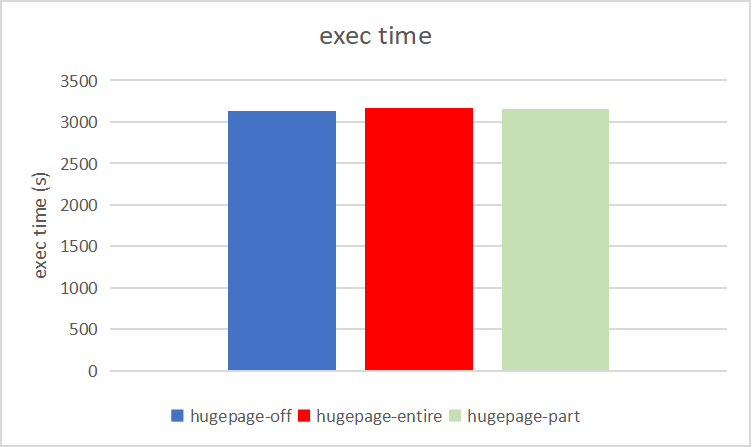
\includegraphics[scale=0.7]{figure/experiment_en/syuron/gmm/exec_time.png}
	\end{minipage}
	\begin{minipage}{0.5\hsize}
  		\centering
		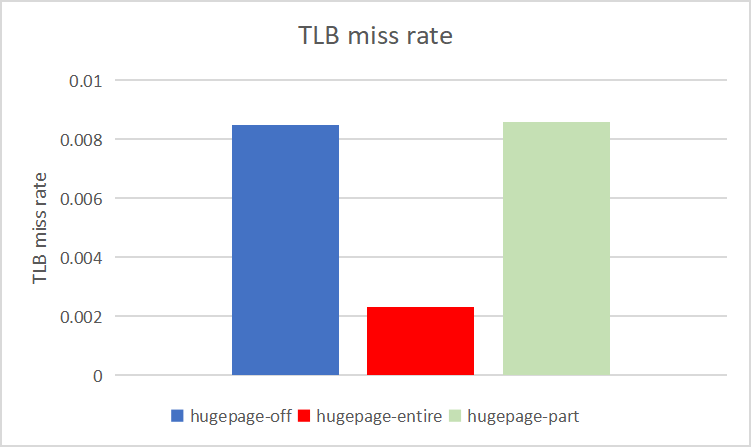
\includegraphics[scale=0.7]{figure/experiment_en/syuron/gmm/tlb_miss.png}
	\end{minipage}
	\\
	\\
	\begin{minipage}{0.5\hsize}
		\centering
	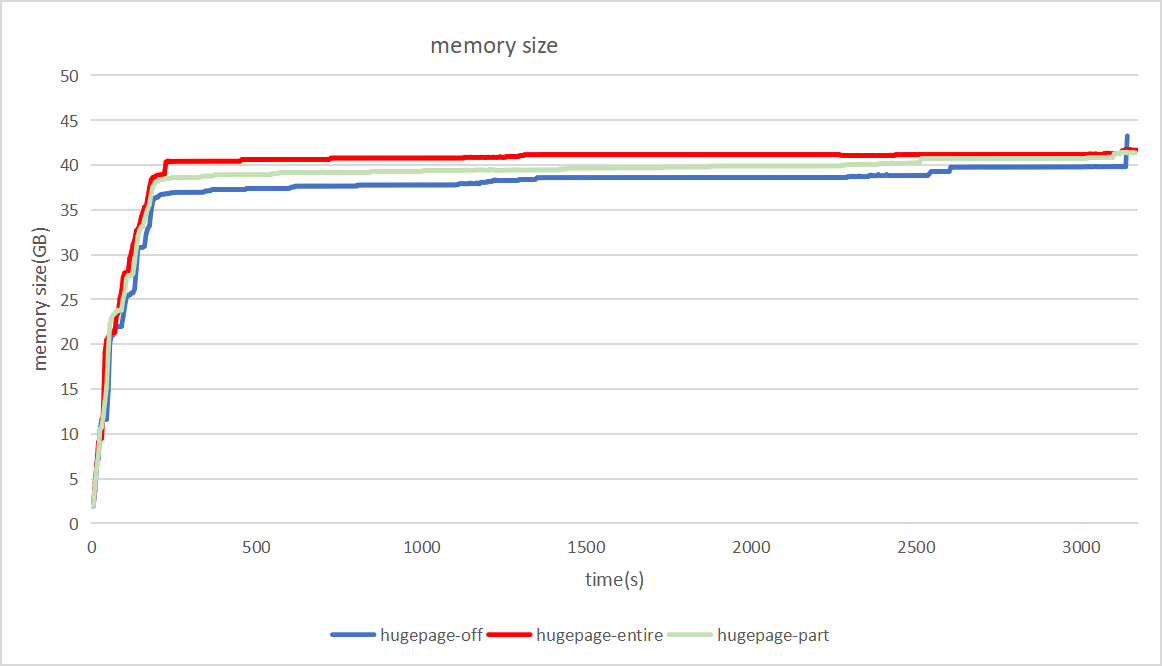
\includegraphics[scale=0.45]{figure/experiment_en/syuron/gmm/memory_size.png}
	\end{minipage}
	\begin{minipage}{0.5\hsize}
		\centering
		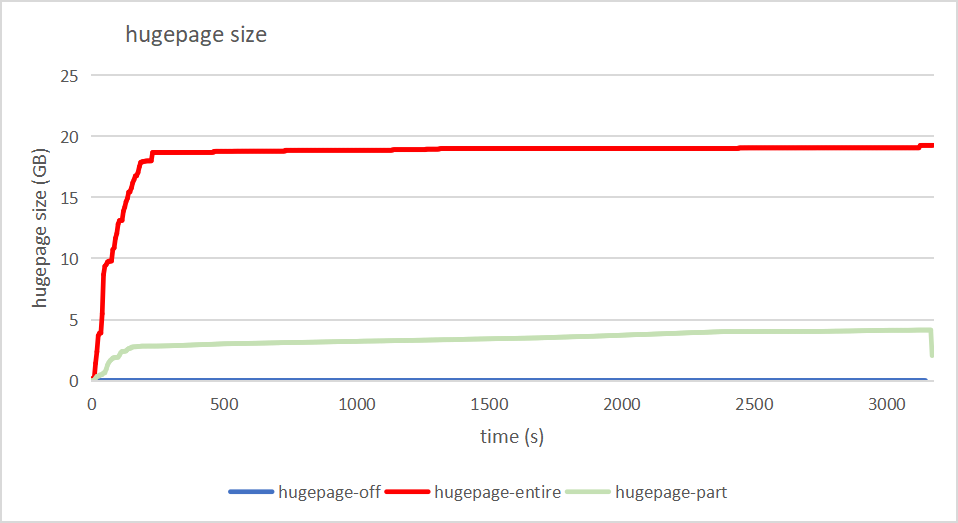
\includegraphics[scale=0.55]{figure/experiment_en/syuron/gmm/hugepage_size.png}
	\end{minipage}
	\caption{experiment result of GMM}
	\label{fig:gmm}
\end{figure}
\subsection{GBT}
The results of the GBT runs are shown in Figure \ref{fig:gbt}.
The execution time shows a reduction of about 13\% for the entire allocation and an increase of about 14\% for the partial allocation. 
In entire allocation, the execution time is thought to have been reduced by speeding up access to HashMap data in the shuffling process, similar to PageRank.
The reason is thought for the large increase in execution time for partial allocation is that memory fragmentation increases due to the large number of shuffles, causing compaction stalls, and the size of the shuffled data to be read/written per iteration changes rapidly, resulting in a large change in disk I/O time.
The memory size is greatly bloat to 17.5GB in the entire allocation, while memory enlargement is suppressed to 8.5GB in the partial allocation, about half of the overall allocation.
\begin{figure}
	\begin{minipage}{0.5\hsize}
  		\centering
		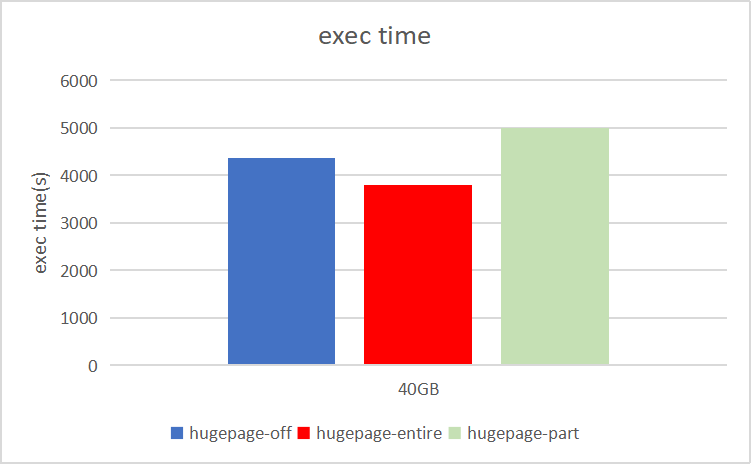
\includegraphics[scale=0.7]{figure/experiment_en/syuron/gbt/exec_time.png}
	\end{minipage}
	\begin{minipage}{0.5\hsize}
  		\centering
		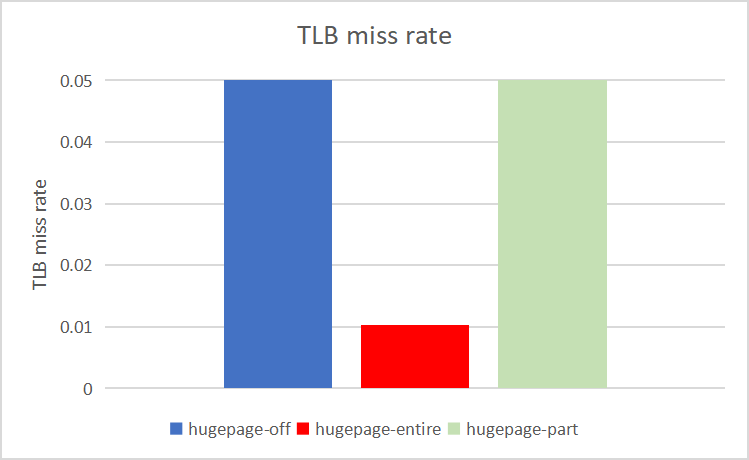
\includegraphics[scale=0.7]{figure/experiment_en/syuron/gbt/tlb_miss.png}
	\end{minipage}
	\\
	\\
	\begin{minipage}{0.5\hsize}
		\centering
	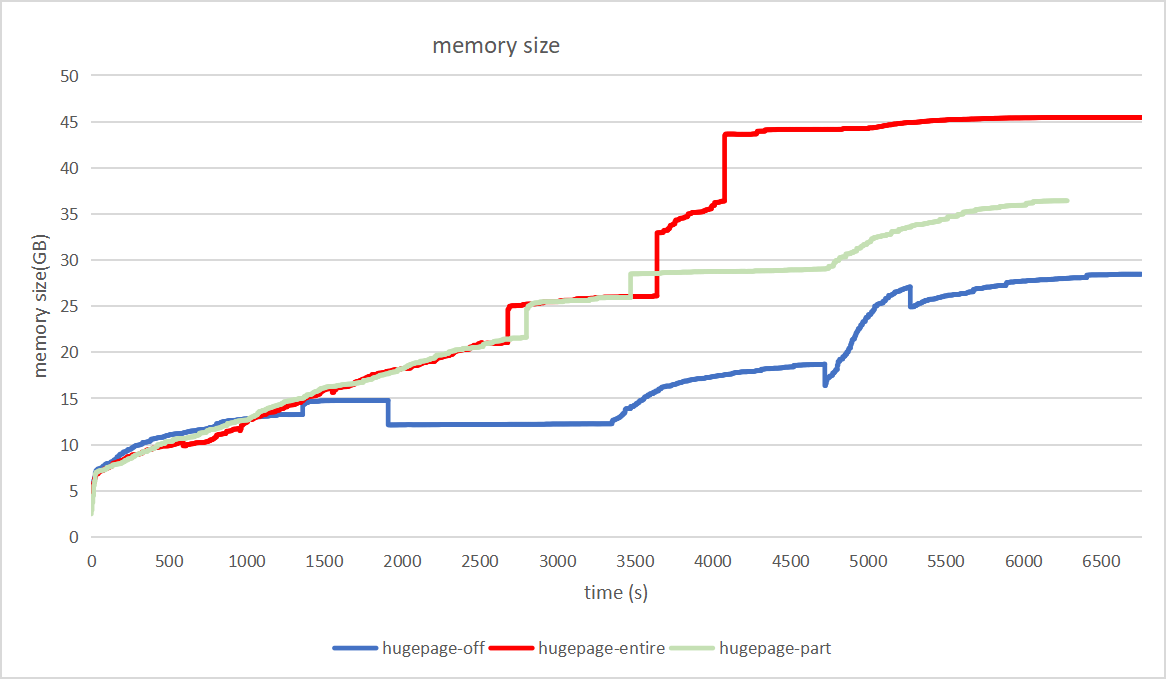
\includegraphics[scale=0.45]{figure/experiment_en/syuron/gbt/memory_size.png}
	\end{minipage}
	\begin{minipage}{0.5\hsize}
		\centering
		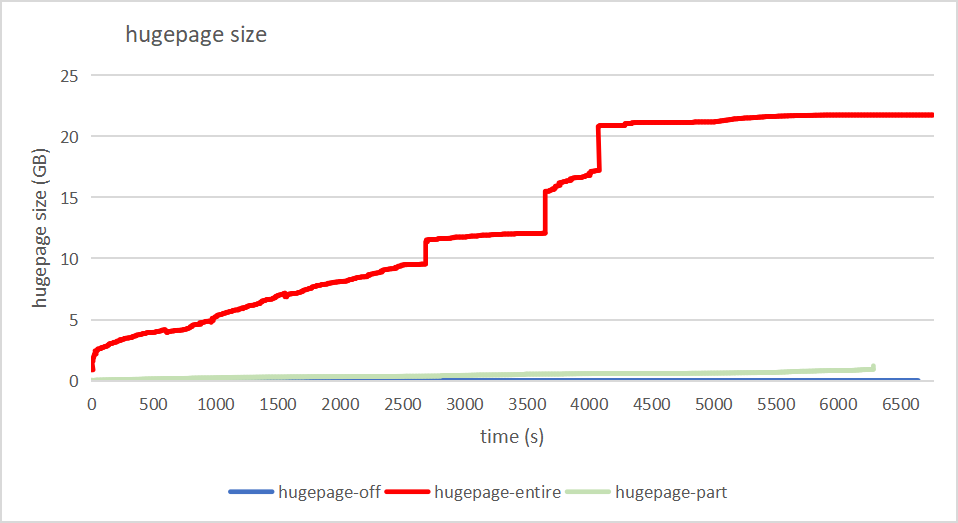
\includegraphics[scale=0.55]{figure/experiment_en/syuron/gbt/hugepage_size.png}
	\end{minipage}
	\caption{experiment result of GBT}
	\label{fig:gbt}
\end{figure}
\subsection{ALS}
The results of the ALS runs are shown in Figure \ref{fig:als}.
The execution time shows that both entire and partial allocations reduce the execution time by approximately 3\%, indicating the effectiveness of HugePages. 
Looking at the TLB misses, the overall allocation was reduced slightly and the partial allocation was not reduced, It is thought that the reduction in execution time was mainly due to the speedup achieved by shortening the page table walk.
Although the data size is small, the number of times the cache is accessed is large, and this is thought that memory access is faster by hugepage for both entire and partial allocations.
The memory size of the entire allocation is about 1GB in the middle of the run, and the memory size of partial allocations is almost completely suppressed, but at the end of the run, entire allocations are bloated.
This is thought to be due to memory requests that can not fill a single Hugepage Region well, wasting the Region and resulting in a rapid increase in memory size.

\begin{figure}
	\begin{minipage}{0.5\hsize}
  		\centering
		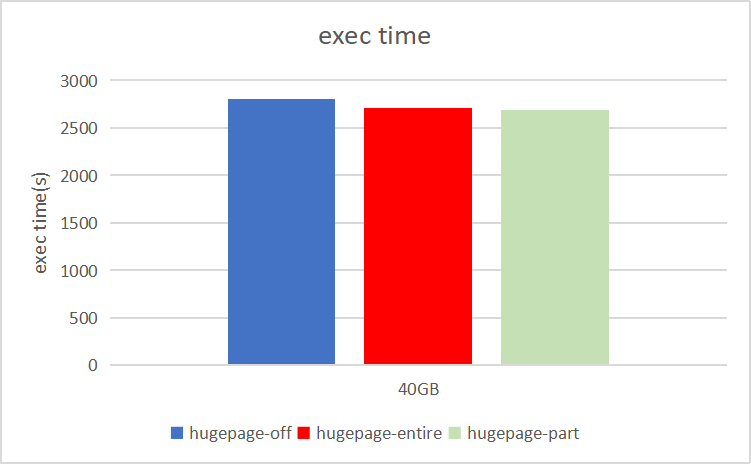
\includegraphics[scale=0.7]{figure/experiment_en/syuron/als/exec_time.png}
	\end{minipage}
	\begin{minipage}{0.5\hsize}
  		\centering
		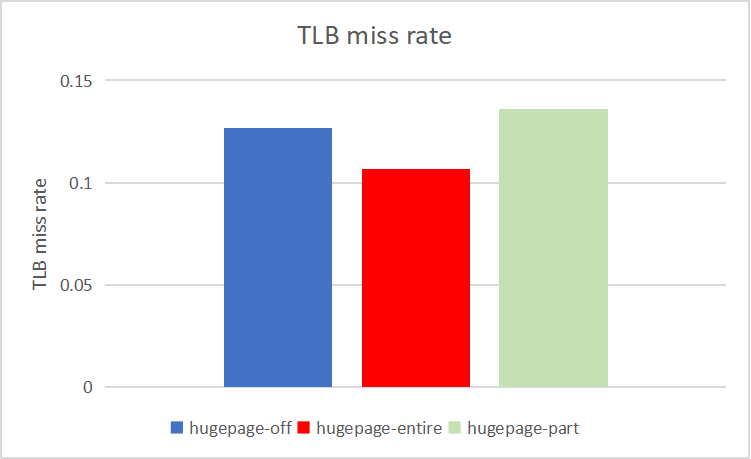
\includegraphics[scale=0.7]{figure/experiment_en/syuron/als/tlb_miss.png}
	\end{minipage}
	\\
	\\
	\begin{minipage}{0.5\hsize}
		\centering
	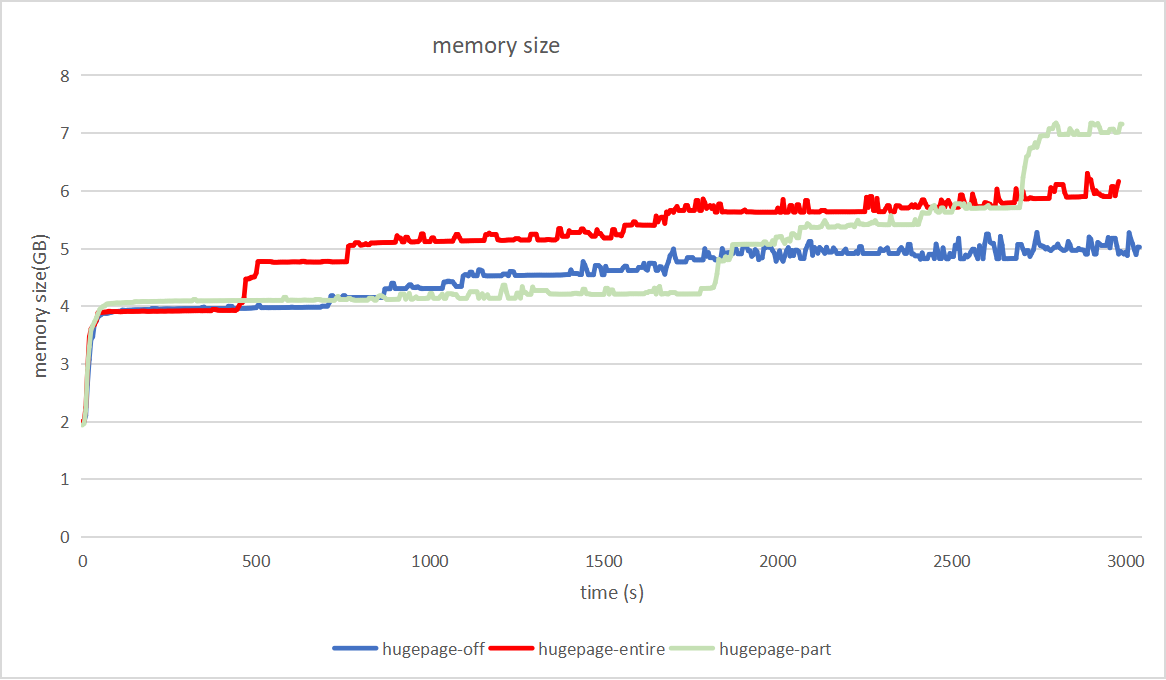
\includegraphics[scale=0.45]{figure/experiment_en/syuron/als/memory_size.png}
	\end{minipage}
	\begin{minipage}{0.5\hsize}
		\centering
		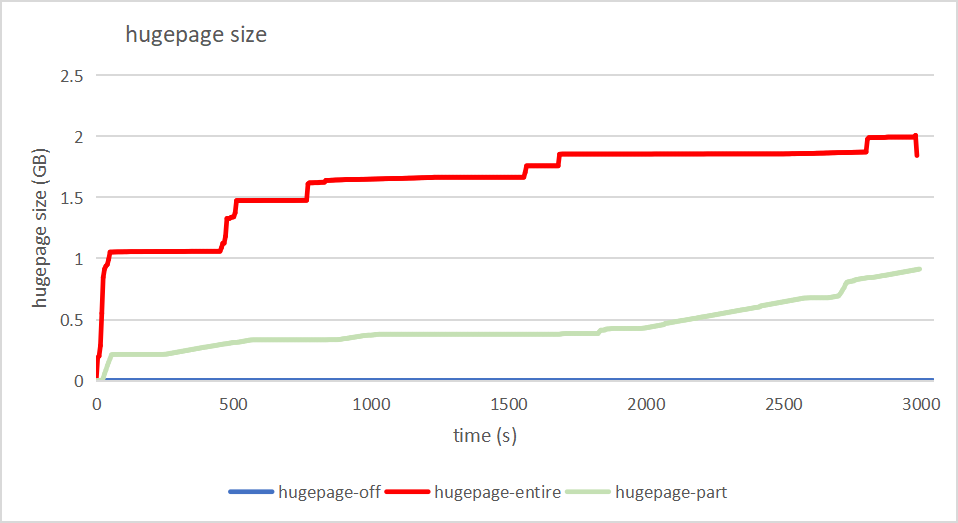
\includegraphics[scale=0.55]{figure/experiment_en/syuron/als/hugepage_size.png}
	\end{minipage}
	\caption{experiment result of ALS}
	\label{fig:als}
\end{figure}
\subsection{SVM}
The results of the SVM runs are shown in Figure \ref{fig:svm}.
The execution time is almost the same for all policies, indicating that there is no effect of the hugepage.
One possible reason is that the data size is so large that disk I/O time becomes long and dominant due to the exchange of a large amount of data even in shuffling, and the benefit of faster memory access becomes almost invisible.
The memory size of the total allocation is enlarged by a maximum of 2.5GB, while that of the partial allocation is bloated by 0.8GB. The entire allocation with a allocat large number of hugepages results in a large memory bloat.
\begin{figure}
	\begin{minipage}{0.5\hsize}
  		\centering
		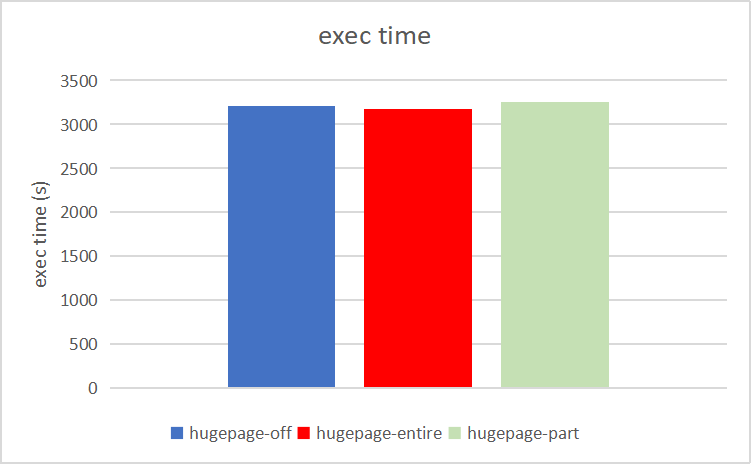
\includegraphics[scale=0.7]{figure/experiment_en/syuron/svm/exec_time.png}
	\end{minipage}
	\begin{minipage}{0.5\hsize}
  		\centering
		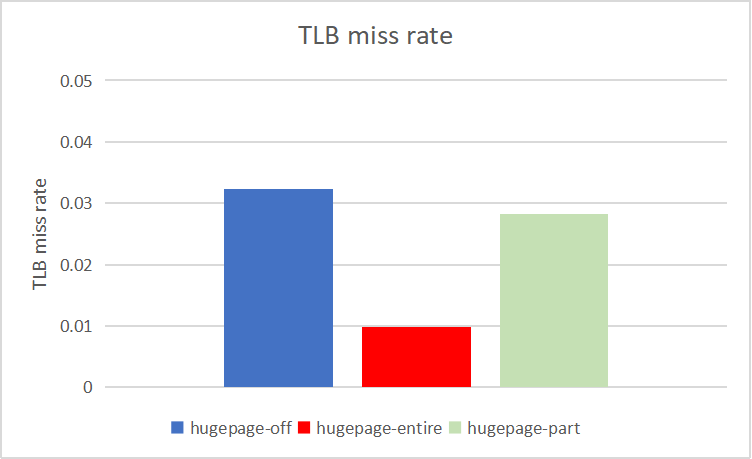
\includegraphics[scale=0.7]{figure/experiment_en/syuron/svm/tlb_miss.png}
	\end{minipage}
	\\
	\\
	\begin{minipage}{0.5\hsize}
		\centering
	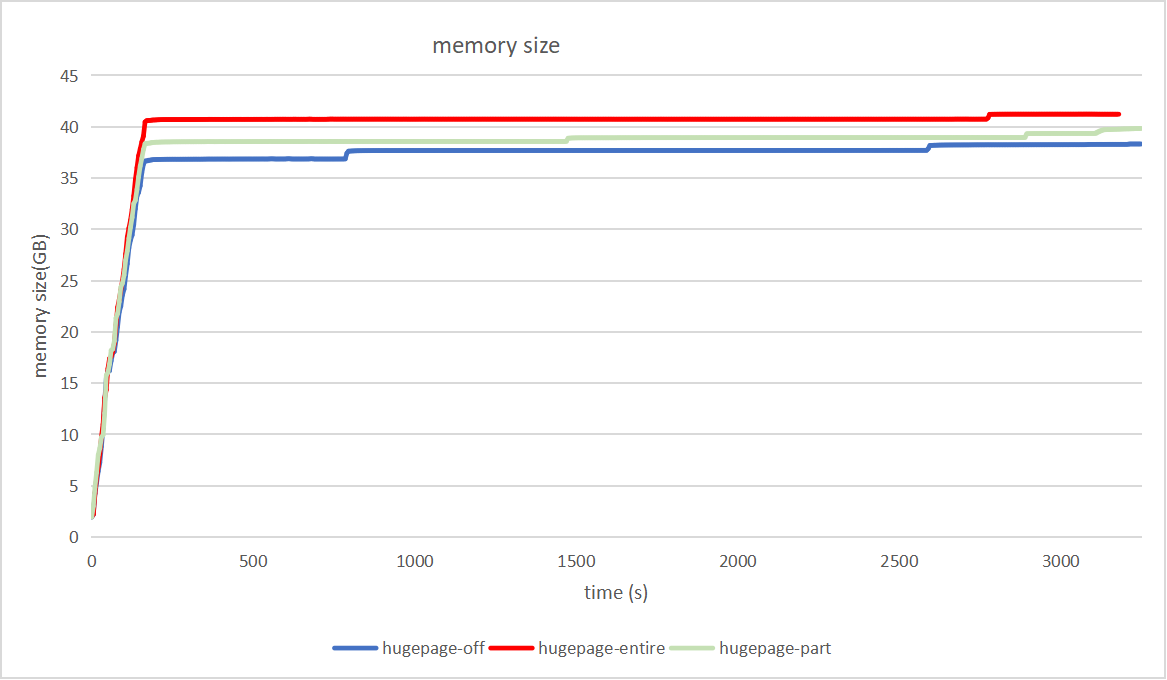
\includegraphics[scale=0.45]{figure/experiment_en/syuron/svm/memory_size.png}
	\end{minipage}
	\begin{minipage}{0.5\hsize}
		\centering
		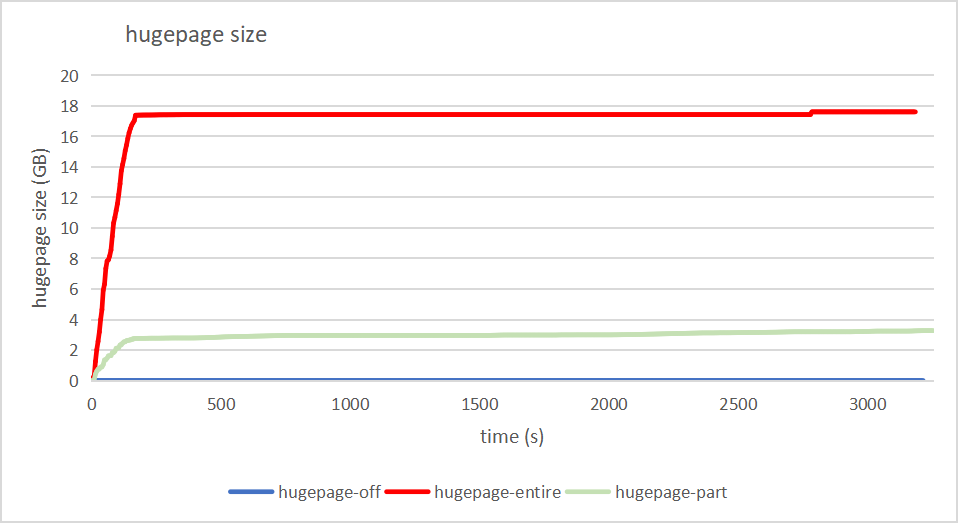
\includegraphics[scale=0.55]{figure/experiment_en/syuron/svm/hugepage_size.png}
	\end{minipage}
	\caption{experiment result of SVM}
	\label{fig:svm}
\end{figure}

\subsection{TC}
The results of the TC runs are shown in Figure \ref{fig:tc}.
In terms of execution time, the overall allocation reduces execution time by approximately 7\%, while the partial allocation is equivalent to no allocation.
The reason is that TLB misses were 0.3\%, and while the overall allocation reduced TLB misses, the partial allocation was not able to reduce TLB misses because the cache size was small and the few hugepage allocation.
The results show that there are many data accesses to ExecutionMemory.
Looking at the memory size, the entire allocation is bloated by up to 4GB, while the partial allocation is almost the same as without allocation, and the hugepage allocation size is also small, indicating that very little StorageMemory is used.
\begin{figure}
	\begin{minipage}{0.5\hsize}
  		\centering
		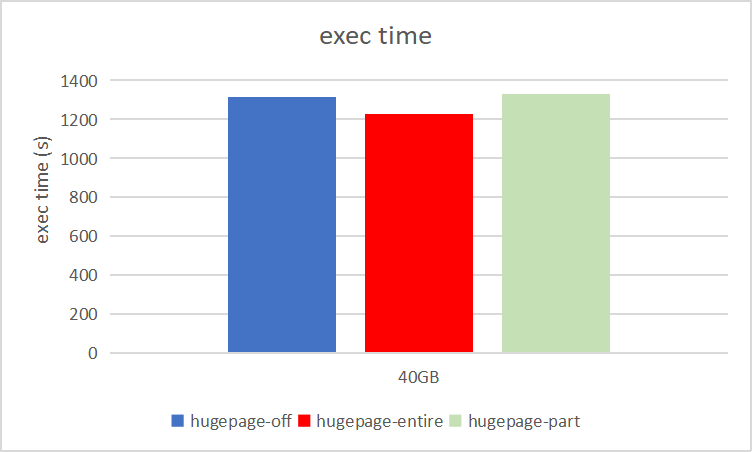
\includegraphics[scale=0.7]{figure/experiment_en/syuron/tc/exec_time.png}
	\end{minipage}
	\begin{minipage}{0.5\hsize}
  		\centering
		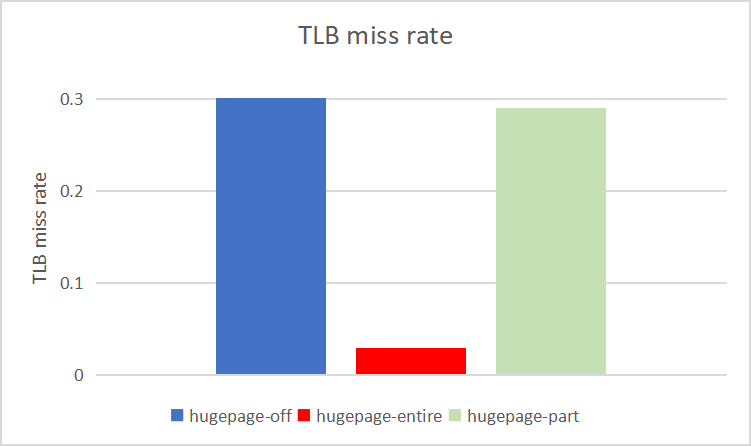
\includegraphics[scale=0.7]{figure/experiment_en/syuron/tc/tlb_miss.png}
	\end{minipage}
	\\
	\\
	\begin{minipage}{0.5\hsize}
		\centering
	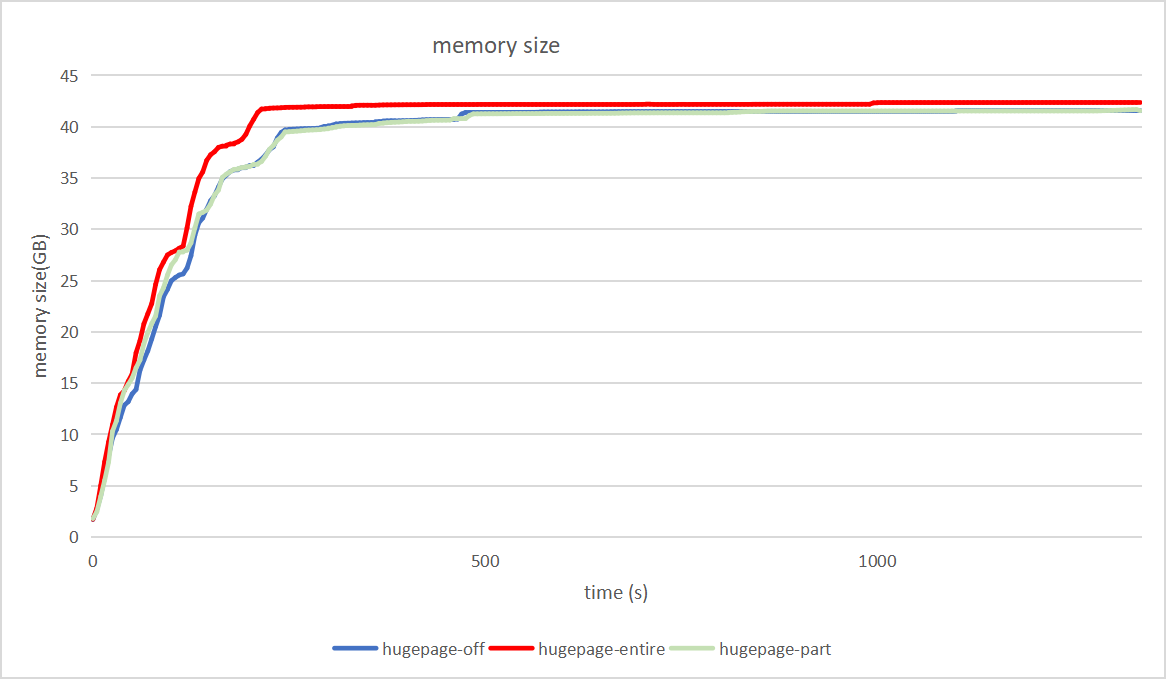
\includegraphics[scale=0.45]{figure/experiment_en/syuron/tc/memory_size.png}
	\end{minipage}
	\begin{minipage}{0.5\hsize}
		\centering
		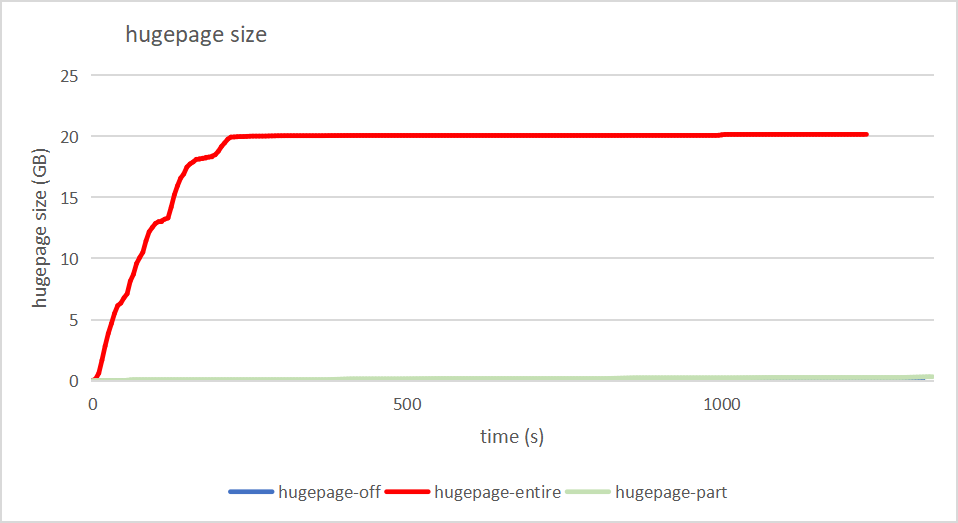
\includegraphics[scale=0.55]{figure/experiment_en/syuron/tc/hugepage_size.png}
	\end{minipage}
	\caption{experiment result of TC}
	\label{fig:tc}
\end{figure}
\section{Discussion}
\subsection{Effect of hugepage in spark}
The experimental results showed that hugepages reduced execution time by up to approximately 13\%, confirming that hugepages The speedup was confirmed.
The execution time was reduced by assigning a hugepage for 7 out of 10 real-world benchmarks, indicating that hugepages are effective for many benchmarks. 
In addition to the execution time reduction achieved by hugh pages for benchmarks with high original TLB miss rates, execution time was also reduced for benchmarks where the original TLB misses were not very high or where the TLB misses were not reduced very much.
This indicates that the effect of hue pages is not only the speedup due to the higher TLB miss rate, but also the speedup due to the shorter page table walk.
In all benchmarks, the use of entire allocation increases memory usage compared to no allocation, with a maximum memory gain of more than 17GB.
In this experimental environment, there were some benchmarks in which the final effect of bloat was eliminated by using up the maximum amount of memory. However, if the system has enough memory, memory bloat may become more serious. 
Memory bloat is thought to be caused by fragmentation due to the use of hugepages.
However, even when comparing between benchmarks with hugepage allocations of around 20GB, memory bloat varies significantly from 4GB to around 17GB.
This is thought to be due to the fact that the size and timing of object generation differs from benchmark to benchmark, and the degree of fragmentation also differs. 
As a result, we found that hugepage allocation is essentially a trade-off between execution time reduction and memory bloat.
In addition, some benchmarks, such as LinearRegression, GMM, and SVM, were found to result in memory bloat despite the lack of execution time reduction.

\subsection{Effect of partial allocation}
Experimental results show that allocation to StorageMemory reduces the execution time of the microbenchmark and LogisticRegression compared to entire allocation, while Kmeasn, ALS, and SVD++ have execution times close to entire allocation, indicating that partial allocation is effect for some real-world benchmarks.
In particular, both the microbenchmark and LogsticRegression do not shuffle, and the LogsticRegression does not shuffle, ExecutionMemory is accessed extremely infrequently, so allocating a hugepage to StorageMemory only is the highest efficient, and the execution time is less than the entire allocation, with less memory bloat. 
However, the execution time was not reduced in benchmarks such as LineareReggression and GMM, where the effect of hugepages was thought to be significant due to the large cache size.
this result show that it is thought that difficult to determine the allocation based on the size of the data stored in StorageMemory alone, and it is important to consider the access frequency and the ratio with other data.
For memory size, except for ALS and LinearRegression, partial allocation could reduce memory bloat compared to entire allocation. 
In terms of memory size, with the exception of ALS and LinearRegression, partial allocation smaller memory size than entire allocation, indicating that memory bloat can be suppressed by reducing the amount of hugepage allocation.
In addition, benchmarks such as PageRank show that total In addition, in benchmarks such as PageRank, the entire allocation reduced execution time, whereas the partial allocation was almost the same as no allocation. Therefore, it is thought that in such benchmarks, allocating hugepages only to ExecutionMemory In such benchmarks, we believe that allocating fusee pages only to ExecutionMemory can achieve the same execution time as overall allocation while minimizing memory bloat.

\subsection{Applications suitable for hugepage}
Based on the results of microbenchmarks, ALS, PageRank, etc., the characteristics of applications that can benefit from the speed-up by HugePages include: large cache data relative to the total memory used by the application, frequent access to cache data, and large data read/write during shuffling.
Benchmarks with high TLB miss ratios were able to reduce execution time. However, benchmarks with low TLB miss ratio could also reduce execution time in some cases, and benchmarks with low TLB miss ratio but with the above characteristics could benefit from hugepages by speeding up the process through page table walks.
On the other hand, if the number of shuffles is too large, the execution time cannot be reduced and only the memory size is bloated, so the disadvantages of hugepage are considered larger when disk I/O is dominant.
Therefore, it is thought that applications in hugepage can reduce execution time, as PageRank does, by shuffling as much as possible at one time.
In the case of short execution times, such as LinearRegression, the execution time has not been reduced, and therefore, it is thought that the hugepage effect would be greater if the application is created to perform one long execution instead of multiple short executions.
It has been confirmed that the memory size can be reduced to some extent by allocating hugepage only a portion of the memory, and it is thought that effective fuse page allocation can be achieved by selecting the range of hugepage allocation. 
In addition, there are cases in which Spark applications are not used repeatedly, but are cached only to ensure fault tolerance.
In this case, the allocation to StorageMemory only does not work well, so it is thought that the benefit of the hugepage by partial allocation can be increased by minimizing the cache to ensure fault tolerance and caching every few dozen loops instead of every single loop. 

\section{Conclusion}
This study investigates the effect of hugh pages in an in-memory distributed processing framework.
To verify the effect of hugepages on Spark's unique memory structure, we implemented a mechanism that allows per-object hugepages to be allocated and conducted experiments using this mechanism in Spark.
The study runs microbenchmarks and 10 real-world benchmarks with three hugepage allocation policies: no hugepage, allocation entire, and partial allocation(only the StorageMemory to Spark).
Experimental results show that HugePages can reduce execution time by up to 13\%.
The maximum memory usage increases by approximately 17GB, and it was found that large memory bloat may occur due to the use of hugepages. 
Partial allocation was found to reduce memory bloat compared to entire allocation, and for some workloads, it reduced execution time as much as or more than entire allocation, indicating that hugepage allocation to only a portion of the workloads can improve performance more than entire allocation.

\bibliographystyle{IEEEtranS}
\bibliography{IEEEexample}


\end{document}